%%%%%%%%%%%%%%%%%%%%%%%%%%%%%%%%%%%%%%%%%%%%%%%%%%%%%%%%%%%%%%%%%%%%%%%%%%%%%%%
\chapter{Complex Algebraic Geometry and Riemann Surfaces}\label{ch:background}
%%%%%%%%%%%%%%%%%%%%%%%%%%%%%%%%%%%%%%%%%%%%%%%%%%%%%%%%%%%%%%%%%%%%%%%%%%%%%%%

In this chapter we will give a brief overview of Riemann surfaces from the
perspective of complex algebraic geometry. Among the primary references used in
this thesis, Griffiths \cite{Giffiths89} provides one of the most succinct
introductions to the subject without requiring background in algebraic geometry
or algebraic curves and gives solid foundation from which to further explore the
topic. Ueno's \cite{Ueno97} presentation is similar but with more emphasis on
the algebraic perspectives whereas Bliss \cite{bliss} focuses on an analytic
approach, instead. Dubrovin's \cite{Dubrovin81} classical manuscript includes
connections to the Kadomtsev-Petviashvili equation introduced in
\autoref{ch:kp}.

%%%%%%%%%%%%%%%%%%%%%%%%%%%%%%%%%%%%%%%%%%%%%%%%%%%%%%%%%%%%%%%%%%%%%%%%%%%%%%%
\section{Complex Algebraic Geometry}\label{sec:background-complex-algebraic-geometry}
%%%%%%%%%%%%%%%%%%%%%%%%%%%%%%%%%%%%%%%%%%%%%%%%%%%%%%%%%%%%%%%%%%%%%%%%%%%%%%%

We begin with some preliminary constructions and facts from complex algebraic
geometry. This section culminates in the Normalization Theorem which connects
the subject to the study of Riemann surfaces. Although other computational
approaches to Riemann surfaces exist, this connection makes the computational
approach possible later.

%..............................................................................
\subsection{The Projective Line}
%..............................................................................

The primary motivation behind complex projective geometry is to make concrete
the way in which we analyze the behavior of functions, such as polynomials, at
infinity without having to resort to techniques separate from those used at
finite points. For example, in applications we may need to integrate a
differential along a path on an algebraic curve going to infinity. Knowing the
geometry of the curve at infinity makes such an operation computationally
feasible.

In fact, anyone with an elementary complex analysis background has seen an
example of projective geometry. The Riemann sphere is the complex plane $\CC$
with a ``point at infinity'' added. Let $z$ denote the coordinate in $\CC$
(i.e., the point $z=0$ represents the origin of the complex plane). In order to
discuss the point at infinity we introduce the coordinate $w = 1/z$. The
analysis of some function at $\infty$ is equivalent to rewriting the problem in
terms of the coordinate $w$ and examining its behavior in a neighborhood of
$w=0$. This explains why, for example, the exponential function
\[
  e^z = \sum_{n=0}^\infty z^n / n!,
\]
though entire in the complex plane, has an essential singularity on the Riemann
sphere since the exponential function in the coordinate $w$ centered at $w=0$ is
expressed by the series
\[
  \sum_{n=0}^\infty \frac{w^{-n}}{n!}.
\]

This point at infinity is not rigorously defined because it does not make sense
to {\it equate} $z=\infty$. The definition of the Riemann sphere is made
explicit by the following construction: consider the set $U = \CC^2 -
\{(0,0)\}$. Define the equivalence relation
\[
  (a_0, a_1) \sim (\lambda a_0, \lambda a_1), \quad \forall \lambda \in \CC -
  \{0\}.
\]
Thus two points $(a_0,a_1)$ and $(b_0,b_1)$ in $U$ are considered the same if
the ratios $a_0 : a_1$ and $b_0 : b_1$ are equal. The set of all points
$(b_0,b_1)$ equal to $(a_0,a_1)$ is called the {\it equivalence class} of
$(a_0,a_1)$ and the {\it complex projective line} $\PP{1}\CC$ is the set of all
such equivalence classes. That is,
\[
  \PP{1}\CC := \CC^2 / \sim.
\]
The equivalence class of $(a_0,a_1)$, called a ``point'' in $\PP{1}\CC$, is
written $(a_0 : a_1) \in \PP{1}\CC$. $\PP{1}\CC$ is precisely the Riemann
sphere. To see this, consider the two subsets
\begin{align*}
  U_0 &= \{ (a_0 : a_1) \in \PP{1}\CC \; | \; a_0 \neq 0 \}, \\
  U_1 &= \{ (a_0 : a_1) \in \PP{1}\CC \; | \; a_1 \neq 0 \}.
\end{align*}
For any $(a_0 : a_1) \in U_0$ we have, by the equivalence property,
\[
  (a_0 : a_1) = (1 : a_1/a_0) = (1 : a).
\]
Similarly, $(b_0 : b_1) = (b : 1)$ for every point in $U_1$. Every point in the
intersection $U_0 \cap U_1$ can be written in either of these two forms. Each of
these subspaces are isomorphic to $\CC$ since the maps
\begin{align*}
  \phi_0 : U_0 \to \CC,
  \quad
  \phi_0 \left( (a_0 : a_1) \right) = a_1 / a_0,
  & \quad \text{ and } \\
  \phi_1 : U_1 \to \CC,
  \quad
  \phi_1 \left( (a_0 : a_1) \right) = a_0 / a_1, &
\end{align*}
are continuous bijections with inverses
\begin{gather}
  \phi^{-1}_0(a) = (1 : a), \\
  \phi^{-1}_1(b) = (b : 1).
\end{gather}
Finally, note that $(0 : 1)$ is the only projective point in $U_1$ which is not
in $U_0$. Therefore, we identify $U_0$ with the complex plane (in the coordinate
$z$) and the point $P_\infty = (0 : 1)$ with the point at infinity and set
\begin{equation} \label{eqn: projective-line}
  \PP{1}\CC = U_0 \cup \{ (0 : 1) \} \cong \CC \cup P_\infty.
\end{equation}

Indeed $P_\infty$ is considered the point at infinity on the Riemann sphere for
if one considers the image of $(0 : 1)$ under $\phi_0$, though undefined since
$(0:1) \not \in U_0$, it maps to $z = 1 / 0$ ``='' $\infty$. Again, this does
not make sense without the complex projective space construction above but is
merely used to illustrate the point. The coordinate transformation from $z$ to
$w$ at the beginning of this section is equivalent to identifying $U_1$ with the
complex plane $\CC$ and $\{(1 : 0)\}$ with the point at infinity, instead.

%------------------------------------------------------------------------------
\subsection{The Projective Plane} \label{sec:projective-plane}
%------------------------------------------------------------------------------

The natural environment we use in the sequel is not the complex projective line
but the complex projective plane. In this section we construct the projective
plane and examine its geometric properties. The construction is similar to that
of the projective line.

Let $U = \CC^3 - \{(0,0,0)\}$. Following the strategy of the previous section,
consider the set of all ratios $(a_0 : a_1 : a_2)$, that is, the collection of
all equivalence classes under the equivalence relation $(a_0 : a_1 : a_2) \sim
(\lambda a_0 : \lambda a_1 : \lambda a_2), \forall \lambda \in \CC - \{0\}$. The
space of all such equivalence classes is called the two-dimensional complex
projective space or {\it the projective plane} and is denoted $\PP{2}\CC$.

Define the subsets $U_0,U_1,U_2$ by
\[
  U_j = \{ (a_0 : a_1 : a_2) \in \PP{2}\CC \; | \; a_j \neq 0 \},
\]
and note that all $(a_0 : a_1 : a_2) \in U_0$ satisfy $(a_0 : a_1 : a_2) = (1 :
a_1/a_0 : a_2/a_0)$. We define the bijective mapping
\begin{gather*}
  \phi_0 : U_0 \to \CC^2, \\
  \phi_0 \left( (a_0 : a_1 : a_2) \right) =
  \left( \frac{a_1}{a_0}, \frac{a_2}{a_0} \right), \\
  \phi_0^{-1} \left( (x,y) \right) = (1 : x : y).
\end{gather*}
The mappings $\phi_1$ and $\phi_2$ are similarly defined on $U_1$ and $U_2$,
respectively. Therefore, we can identify $U_0$ with the complex plane $\CC^2$.

Consider the space $U_0^c = \PP{2}\CC - U_0$. By definition, every point in
$U_0^c$ is of the form $(0 : a_1 : a_2)$. By definition, every point in $U_0^c$
determines a point on the complex projective line $\PP{1}\CC$. The converse is
true as well, resulting in the bijection
\[
  (0 : a_1 : a_2) \in \PP{2}\CC \; \leftrightarrow \; (a_1 : a_2) \in \PP{1}\CC.
\]
By identifying $U_0^c$ with $\PP{1}\CC$ we may write
\begin{equation} \label{eqn: proejctive-plane} \PP{2}\CC = U_0 \cup U_0^c \cong
  \CC^2 \cup \PP{1}\CC
\end{equation}
where $U_0^c \cong \PP{1}\CC$ is called the {\it line at infinity}, denoted
$l_\infty$, and $U_0 \cong \CC^2$ is called the {\it complex affine plane}. We
may also identify the complex affine plane with the sets $U_1$ or $U_2$ and the
line at infinity with their complements.

We saw a natural geometric interpretation of $\PP{1}\CC$ in the previous
section. Does such an interpretation exist for $\PP{2}\CC$? Consider a line in
the complex affine plane $\CC^2$ which can be written in the form
\[
  \alpha + \beta x + \gamma y = 0, \quad \text{where } (\beta,\gamma) \neq 0,
  \alpha, \beta, \gamma \in \CC.
\]
Using the inverse mapping $\phi_0^{-1}$ on $\CC^2$ we have
\[
  x = \frac{x_1}{x_0} \text{ and } y = \frac{x_2}{x_0},
\]
where $(x_0 : x_1 : x_2)$ are the coordinates of $\PP{2}\CC$, and we get the
line
\[
  \alpha x_0 + \beta x_1 + \gamma x_2 = 0.
\]
This equation, called the {\it homogenization} of the affine curve, makes sense
in all of $\PP{2}\CC$. Setting $x_0 = 1$ gives the original affine line. On the
other hand, setting $x_0 = 0$ gives the equation
\[
  \beta x_1 + \gamma x_2 = 0,
\]
which is the equation of the line in $l_\infty$. However, this implies $x_1 /
x_2 = - \gamma / \beta$. Hence the projective point $(0 : -\gamma : \beta)$
satisfies the equation
\[
  \alpha x_0 + \beta x_1 + \gamma x_2 = 0
\]
and is, in fact, the only projective point in $l_\infty$ on the line.

This means that the line ``intersects'' $l_\infty$ at the point $(0 : -\gamma :
\beta)$ and that this intersection point depends only on the slope of the affine
portion of the line. Hence, the line at infinity has the geometric meaning that
each point on it is the intersection point of an entire family of parallel lines
in $\CC^2$. This leads to a generalization of a theorem from classical planar
geometry: {\it any two, distinct lines in $\PP{2}\CC$ intersect at exactly one
  point}.

%------------------------------------------------------------------------------
\subsection{Projective Plane Curves} \label{sec: projective-plane-curves}
%------------------------------------------------------------------------------

The set of all points $(x_0, x_1, x_2)$ satisfying
\[
  \alpha x_0 + \beta x_1 + \gamma x_2 = 0
\]
is called a {\it projective line} and is a simple example of a projective
algebraic curve (of degree one). In this section we introduce various properties
of general projective curves.

A {\it complex plane algebraic curve} is the zero locus of the homogenization of
a polynomial $f \in \CC[x,y]$. That is, given a polynomial $f(x,y) = \alpha_n(x)
y^n + \alpha_{n-1}(x)y^{n-1} + \cdots + \alpha_0(x)$ its homogenization is the
polynomial $F \in \PP{2}\CC[x_0,x_1,x_2]$ where
\[
  F(x_0,x_1,x_2) = x_0^d f(x_1/x_0,x_2/x_0),
\]
and where $d$ is the degree of $F$. The homogeneity of $F$ means that we can
write,
\[
  F(x_0,x_1,x_2) = \sum_{i+j+k=d} \alpha_{ijk} x_0^i x_1^j x_2^k.
\]

In terms of the projective polynomial $F$, its affine part can be written
$F(x,y) = F(1,x,y)$. As in the case of a projective line, $f$ can be thought of
as a projection of the polynomial $F$ onto $\CC^2$ and there is always a
one-to-one correspondence between an affine polynomial and its homogenization.
Therefore, a {\it complex plane algebraic curve} is the set
\[
  C = \left\{ (x_0 : x_1 : x_2) \in \PP{2}\CC : F(x_0,x_1,x_2) = 0 \right\}.
\]

Important to the study of projective curves, and specifically in the
computational work described here, are singular points.
\begin{definition} \label{def: singular-point} A point $a = (a_0 : a_1 : a_2)
  \in C$ is a {\bf singular point of $C$}, or a {\it multiple point of $C$}, if
  \[
    \left( \frac{\partial F}{\partial x_0},
      \frac{\partial F}{\partial x_1},
      \frac{\partial F}{\partial x_2} \right) (a) = (0,0,0).
  \]
\end{definition}
Consider the case when $a = (1 : 0 : 0)$ (corresponding to the point $(0,0)$ in
the affine plane $\CC^2$) is a singular point of $F$. The affine poirtion of the
curve is
\[
  f(x,y) = \sum_{i+j \geq 2}^d c_{ij} x^iy^j.
\]
Note that the constant term is zero since $(0, 0)$ is a point on the affine
curve and the linear term vanishes since $(0,0)$ is a singular point. We write
\[
  f(x,y) = f_m(x,y) + f_{m+1}(x,y) + \cdots + f_d(x,y), \quad m \geq 2,
\]
where each $f_n$ is the sum of all terms of $f$ of degree $n$; that is, terms of
the form $c_{ij}x^iy^j$ such that $i+j=n$. The smallest such $m$ with non-zero
term $f_m$ appearing in $f$ is called the {\it multiplicity} of the singular
point $(1 : 0 : 0)$. Singularities with multiplicity two are called {\it double
  points}, those with multiplicity three are called {\it triple points}, and so
on.

The homogeneous term $f_m$ can be factored into linear factors,
\[
  f_m(x,y) = \prod_{j=1}^m (\alpha_j x - \beta_j y).
\]
We call the space $C_m = \{(x,y) \in \CC^2 : f_m(x,y) = 0\}$ the {\it tangent
  cone of the plane curve $C$} at $a = (1 : 0 : 0)$ which consists of a finite
number of intersecting lines $L_j : \alpha_j x - \beta_j y$.

When a generic affine point $a = (1 : c : d)$ is a singular point we write the
affine curve in the form,
\[
  f(x,y) = \sum_{i+j \geq 2}^d \tilde{c}_{ij} (x-c)^i(y-d)^j,
\]
which we can write as a sum of polynomials $g_n(x-c,y-d)$ homogenous in $x-c$
and $y-d$.

In the case when the singular point $a = (0 : 1 : b) \in l_\infty$ we repeat the
above process with the affine curve,
\[
  g(u,v) = \frac{1}{x_1^d} F(x_0, x_1, x_2) = F(u,1,v), \quad u =
  \frac{x_0}{x_1}, v = \frac{x_2}{x_1},
\]
which is a projection of $F$ onto $U_1 \cong \CC$ instead of $U_0$. We write $g$
as a sum of terms of the form $g_{ij}u^i(v-b)^j$. Finally, in the case $a = (0 :
0 : 1) \in l_\infty$ we use the affine curve
\[
  h(w,z) = \frac{1}{x_2^d} F(x_0, x_1, x_2) = F(w,z,1), \quad w =
  \frac{x_0}{x_2}, z = \frac{x_1}{x_2},
\]
and write $h$ as a sum of terms of the form $h_{ij}w^iz^j$.

\begin{example} \label{ex: 2-cubic}
Consider the cubic curve
\[
  C: F(x_0,x_1,x_2) = x_0^4 x_2^3 + 2 x_0^3 x_1^3 x_2 - x_1^7
\]
In complex affine space $x_0 = 1$ this curve is
\[
  f(x,y) = F(1,x,y) = y^3 + 2 x^3 y - x^7.
\]
A plot of $f$ for $x,y$ real is shown in Figure \ref{fig: example-cubic}. For $a
= (a_0 : a_1 : a_2)$ we have
\begin{align} \label{eq: singular-conditions}
  \frac{\partial F}{\partial x_0}(a)
  &=
  4 a_{0}^{3} a_{2}^{3} + 6 a_{0}^{2} a_{1}^{3} a_{2}, \notag \\
  \frac{\partial F}{\partial x_1}(a)
  &=
  6 a_{0}^{3} a_{1}^{2} a_{2} - 7 a_{1}^{6}, \notag \\
  \frac{\partial F}{\partial x_2}(a)
  &=
  3 a_{0}^{4} a_{2}^{2} + 2 a_{0}^{3} a_{1}^{3}.
\end{align}

\begin{figure}
  \centering
  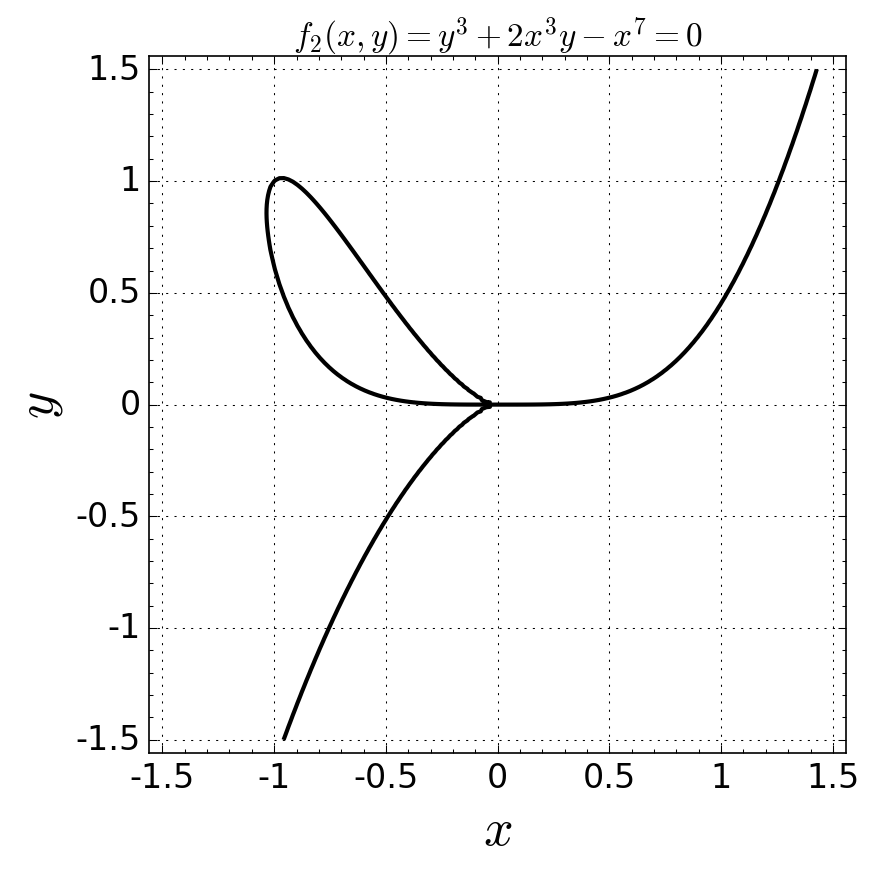
\includegraphics[width=0.5\textwidth]{images/f2.png}
  \caption{A real plot of the curve $C : f(x,y) = y^3 + 2 x^3 y - x^7$. The plot
    suggests that $(x_0 : x_1 : x_2) = (1 : 0 : 0)$, corresponding to $(x,y) =
    (0,0)$, is a singular point of $C$.}
  \label{fig: example-cubic}
\end{figure}

First, we find the finite singular points of $C$. Setting $a_0=1$ and solving
the above equations for $a_1$ and $a_2$ we see that $p = (1 : 0 : 0)$ is the
only finite singular point of $F$. Note that
\begin{gather*}
  f(x,y) = f_3(x,y) + f_4(x,y) + f_7(x,y), \\
  \\
  f_3(x,y) = y^3, \quad
  f_4(x,y) = 2 x^3 y, \quad
  f_7(x,y) = -x^7,
\end{gather*}
and that $f_3$, $f_4$, and $f_7$ are homogeneous of degrees 3, 4, and 7,
respectively. Therefore, $p$ is a singular point of multiplicity 3 with
\[
  f_3(x,y) = y^3 = 0,
\]
as the equation for the tangent cone at $p$. These properties are suggested by
Figure \ref{fig: example-cubic} where, near the point $p$, the real curve looks
like the intersection of three curves well approximated by the line $y = 0$ near
the point $x = 0$.

Setting $a_0 = 0$, the only expression in Equation \eqref{eq:
  singular-conditions} that does not reduce to zero is
\[
  \frac{\partial F}{\partial x_1}((0,a_1,a_2)) = - 7 a_{1}^{6} = 0,
\]
implying that the point $a = (0 : 0 : 1)$ is the only singular point at
infinity. The curve at infinity centered at $(0 : 0 : 1)$ is
\[
  h(w,z) = F(w,z,1) = w^{4} + 2 w^{3} z^{3} - z^{7}.
\]
The order of this singularity is four since this is the degree of the lowest
degree homogeneous term. The tangent cone at $a$ is $g_4(w,z) = w^4$.
\end{example}


%------------------------------------------------------------------------------
\subsection{Connection to Riemann Surfaces} \label{subsec:connection-to-riemann-surfaces}
%------------------------------------------------------------------------------

There is a close relationship between the study of compact Riemann surfaces and
that of algebraic curves. Recall that a Riemann surface $X$ is a complex
manifold of complex dimension one endowed with an {\it atlas}: an open covering
$\{U_\alpha \}_{\alpha \in A}$ of $X$ together with a collection of
homeomorphisms $\{z_\alpha : U_\alpha \to \CC\}_{\alpha \in A}$, called {\it
  local parameters}, such that every pair of {\it transition functions}
\[
  f_{\beta,\alpha} := z_\beta \circ z_\alpha^{-1} : z_\alpha \left( U_\alpha
    \cap U_\beta \right) \to z_\beta \left( U_\alpha \cap U_\beta \right),
\]
is holomorphic. The pairs $(U_\alpha, z_\alpha)$ are called {\it coordinate
  charts}. In other words, a Riemann surface is a topological space such that
for all $P \in X$ there is a neighborhood of $P$ homeomorphic to an open subset
of the complex plane and one can analytically continue from any $P \in X$ to any
$Q \in X$ via transition functions.

The Riemann sphere $X = \CC^*$ is an example of a Riemann surface. Its atlas
consists of two coordinate charts $(U_1, z_1)$ and $(U_2, z_2)$ with
\begin{align*}
  U_1 = \CC, & \quad z_1 = z, \\
  U_2 = \left( \CC - \{0\} \right) \cup \{ \infty \}, & \quad z_2 = 1/z.
\end{align*}
This is a valid atlas since the transition functions
\begin{gather*}
  f_{1,2}, f_{2,1} : \left(\CC - \{0\}\right)
  \to \left(\CC - \{0\}\right) \\
  f_{1,2} = z_1 \circ z_2^{-1} = 1/z \\
  f_{2,1} = z_2 \circ z_1^{-1} = 1/z
\end{gather*}
are holomorphic on $U_1 \cap U_2 = \CC - \{0\}$.

These relationships between curves and Riemann surfaces are embodied by the
following two theorems % TODO Griffiths reference

\begin{theorem} \label{thm: normalization} {\bf (Normalization Theorem.)} For
  any irreducible algebraic curve $C \subset \PP{2}\CC$ there exists a compact
  Riemann surface $X$ and a holomorphic mapping
  \[
    \sigma : X \to \PP{2}\CC,
  \]
  such that $\sigma( X ) = C$ and $\sigma$ is injective on the inverse image of
  the set of smooth points of $C$.
\end{theorem}

A Riemann surface together with the mapping $\sigma$ is called the {\it
  normalization of $C$}. Loosely speaking, the normalization theorem states that
an algebraic curve is a Riemann surface except at the singular points.

Conversely, every compact Riemann surface can be represented by an algebraic
curve.
\begin{theorem} \label{thm: repr-theorem} Any compact Riemann surface $X$ can be
  obtained through the normalization of a certain plane algebraic curve $C$ with
  at most ordinary double points. That is, there exists a holomorphic mapping
  \[
    \sigma : X \to \PP{2}\CC
  \]
  such that $\sigma(X)$ is an algebraic curve possessing at most ordinary double
  points.
\end{theorem}
Many of the geometric algorithms presented in this document are designed to
avoid singular points. Except, for example, when we want to integrate a 1-form
along a path leading to a singular point in which case we ``unwrap'' the
singularity using Puiseux series. This is discussed in more detail in the
following section. However, because of this we use the terms ``curve'' and
``Riemann surface'' interchangably.

Additionally, the algorithms presented in this document primarily work with the
affine part $f(x,y)$ of the curve $F(x_0,x_1,x_2)$. If analysis on the line at
infinity is necessary, for example, when computing the singular points of a
curve, we consider an affine projection $g$ of $F$ onto $l_\infty$,
\[
  g(u,y) = u^d f(1/u,y) = 0.
\]

Thus, the surface considered here is the branched algebraic $y$-covering of the
complex $x$-Riemann sphere, the set of all $(x,y)$-solutions to the affine
polynomial equation
\[
    C = \{ (x,y) \in \CC \; | \; f(x,y) = \alpha_d(x)y^d +
    \alpha_{d-1}y^{d-1} + \cdots + \alpha_1(x)y + \alpha_0(x) = 0\},
\]
as $x$ varies along all of $\CC$. We treat $x$ and $y$ as the independent and
dependent variables of the equation, respectively.

A {\it point} $\alpha \in \CC$ is called a {\it regular point of $C$} if
\[
  f(\alpha,y) = 0
\]
has $d$ distinct $y$-roots $y_0,\ldots,y_{d-1}$. A point $\alpha \in \CC$ is
called a discriminant point if it is not regular. The point $\alpha = \infty$ is
a regular point of $C$ if
\[
  g(0,y)
\]
has $d$ disctinct roots.

A {\it place} $P$ is an element of $X$. For all but finitely many places, $P$ is
given by a pair $(\alpha,\beta)$ such that $f(\alpha,\beta) = 0$. However, some
places, particularly those where $\alpha$ is a discriminant point, instead needs
to be represented by a pair of series $(x(t),y(t))$ in some local coordinate
$t$. This will be discussed in more detail in the following section.


%%%%%%%%%%%%%%%%%%%%%%%%%%%%%%%%%%%%%%%%%%%%%%%%%%%%%%%%%%%%%%%%%%%%%%%%%%%%%%%
\section{Algebraic Curves and Riemann
  Surfaces}\label{sec:background-algebraic-curves-and-riemann-surfaces}
%%%%%%%%%%%%%%%%%%%%%%%%%%%%%%%%%%%%%%%%%%%%%%%%%%%%%%%%%%%%%%%%%%%%%%%%%%%%%%%

In the previous section we introduced the Normalization Theorem relating complex
algebraic curves to Riemann surfaces. The goal of this section is to derive the
period matrix of a Riemann surface, the Abel Map, and the Riemann theta
function. These three objects are the primary ingredients in constructing a
large class of solutions to the Kadomtsev--Petviashvili equation, discussed in
\autoref{ch:kp}, and determinantal representations of plane curves, discussed in
\autoref{ch:determinantal}.

Throughout this section we present computational examples using the Sage
software package Abelfunctions \cite{abelfunctions}. Abelfunctions is a library
which provides general and easy to use framework for computing with Abelian
functions, Riemann surfaces, and algebraic curves. The reader may follow along
in the computations by downloading and installing Sage \cite{sage} from
\url{www.sagemath.org} and following the instructions on
\url{github.com/abefunctions/abelfunctions} for downloading and installing
Abelfunctions. See \autoref{ch:abelfunctions} for information on the algorithms
used and design of the software. In particular, an algorithmic perspective on
the below components can be found in \autoref{sec:abelfunctions-algorithms}.

\begin{figure}
\centering
\begin{tikzpicture}
  \tikzstyle{element}=[rectangle, rounded corners, thick, draw]
  \tikzstyle{leadsto}=[->, shorten >=5pt, shorten <=5pt, >=latex, thick]

  % period matrix, abel map, and riemann constant vector
  \node[element] (periodmatrix) {Period Matrix};
  %\node[element] (abelmap) {Abel Map};
  %\node[element] (rcv) {Riemann Constant Vector};

  % dummy element to the left of period matrix
  \node[left=of periodmatrix, xshift=-1cm] (dummy) {};

  % = algebraic side =
  \node[element, above=of dummy] (oneforms) {1-Forms}
      edge [leadsto] (periodmatrix);
  \node[left=of oneforms, xshift=-0.5cm] (algdummy) {}; % alg dummy
  \node[element, above=of algdummy] (intbasis) {Integral Basis}
      edge [leadsto] (oneforms);
  \node[element, below=of algdummy] (singularities) {Singularities}
      edge [leadsto] (oneforms);
  \node[element, left=of algdummy,xshift=-0.2cm] (puiseux) {Puiseux Series}
      edge [leadsto] (singularities)
      edge [leadsto] (intbasis);

  % = geometric side =
  \node[element, below=of dummy] (homology) {Homology}
      edge [leadsto] (periodmatrix);
  \node[element, left=of homology] (monodromy) {Monodromy}
      edge [leadsto] (homology);
  \node[element, left=of monodromy, text width=2.5cm, align=center] (ancont) {Analytic Continuation}
      edge [leadsto] (monodromy);
\end{tikzpicture}
\caption{The major computations performed by {\tt abelfunctions} and
  their dependencies on one another.}
\label{fig: dependencies}
\end{figure}


The examples used in this chapter use the curves,
\begin{align}
  C_2 &:  f_2(x,y) = y^3 + 2x^3y - x^7 = 0, \label{eq:example-curve-f2} \\
  C_4 &:  f_4(x,y) = x^2y^3 - x^4 + 1 = 0. \label{eq:example-curve-f4}
\end{align}
In order to execute the code examples used in the rest of this chapter we begin
by starting Sage, importing Abelfunctions, and defining these two curves in
Sage,
\begin{lstlisting}
sage: from abelfunctions import *
sage: R.<x,y> = QQ['x,y']; R
Multivariate Polynomial Ring in x, y over Rational Field
sage: f2 = y^3 + 2*x^3*y - x^7
sage: X2 = RiemannSurface(f2)
sage: f4 = x^2*y^3 - x^4 + 1
sage: X4 = RiemannSurface(f4)
\end{lstlisting}


%%%%%%%%%%%%%%%%%%%%%%%%%%%%%%%%%%%%%%%%%%%%%%%%%%%%%%%%%%%%%%%%%%%%%%%%%%%%%%%
\subsection{Puiseux Series}\label{subsec:background-puiseux-series}
%%%%%%%%%%%%%%%%%%%%%%%%%%%%%%%%%%%%%%%%%%%%%%%%%%%%%%%%%%%%%%%%%%%%%%%%%%%%%%%

% ``From Riemann to Differential Geometry and Relativity''
\begin{quote}
  Victor Puiseux's modesty was intimidating, and his patience and politeness
  were admirable. To a student blundering at some test, he just used to say,
  with a very sweet tone: ``I don't know whether I heard well or whether I am
  mistaken, but it seems to me that what you said is not completely true.'' ---
  \'{E}mile Picard
\end{quote}

Every analytic function $f \in C^1(\RR)$ admits a local Taylor series
representation in a neighborhood about $x = \alpha$. If the function is
meromorphic it still admits a local series representation in the form of a
Laurent series,
\[
    f(x) = \sum_{n=N}^\infty c_n (x-\alpha)^n
\]
for some $N \in \ZZ \cup \{-\infty\}$ depending on $\alpha$. In both of these
situations the variable $x$ is a {\it local coordinate} of $f$ near the point
$\alpha$.

With algebraic curves, local coordinates are given in terms of Puiseux series
which can be thought of as an extension of Laurent series.
\begin{definition} \label{def: puiseux} A {\bf Puiseux series} expansion of a
  curve $C : f(x,y) = 0$ at the point $x=\alpha$ is a collection of $j =
  1,\ldots,m$ series, $m \leq d = \text{deg}_y f$, of the form
  \begin{align*}
    P_j(t) =
    \begin{cases}
      x_j(t) = \alpha + \lambda_j t^{e_j}, \\
      y_j(t) = \sum_{k=N}^\infty \beta_{jk} t^{n_{jk}},
    \end{cases}
  \end{align*}
  where $N \in \ZZ \cup \{-\infty\}$, $\alpha, \lambda_j, \beta_{jk} \in \CC$,
  and $e_j,n_{jk} \in \ZZ$. Each Puiseux series $P_j$ is called a {\bf place} on
  $C$. The variable, $t$, is called the {\bf local parameter} of the series and
  is centered at $t=0$.
\end{definition}
A place $P_j = P_j(t)$ satisfies,
\[
    f\big(P_j(t)\big) := f\big(x_j(t), y_j(t)\big) = 0.
\]
When a Puiseux series $P_j(t)$ represents an expansion about a non-singular
$(\alpha, \beta_j)$ on the curve then $P(0) = (\alpha,\beta)$. This is not
necessarily the case with singular places. We list some additional important
facts and properties of Puiseux series.
\begin{itemize}
\item The integer $|e_j|$ is called the {\it branching number} or {\it
    ramification index} of the series expansion at that place: $|e_j| > 1$ when
  $x = \alpha$ is a branch point of the curve. If $e_j = 1$ we say that the
  place is {\it unramified}.
\item The number of Puiseux series $m$ at a branch point $x = \alpha$ is less
  than or equal to $d = \text{deg}_y f$. In particular, $d = \sum_{j=1}^m
  |e_j|$. If $\alpha$ is not a branch point of the curve (see Section
  \ref{subsec:background-monodromy}) then $e_j = 1$ for all $j = 1, \ldots, d$;
  that is, there are $d$ unramified places above $x = \alpha$.
\item The field of Puiseux series is a splitting field for $\CC[x,y] =
  \CC[x][y]$. That is, given any $f \in \CC[x,y]$ and Puiseux series expansions
  about any $x=\alpha$ we can write
  \[
    f(x,y) = \prod_{j=1}^m \prod_{k=1}^{e_j} \left( y - y_j\left(
             (e/\lambda_j)^{2 \pi ik / e_j}(x-\alpha) \right) \right),
  \]
  where the first product ranges over all Puiseux series $P_j$ at $x=\alpha$ and
  the second product ranges over all $y$-components $y_j(x_j)$ when solving for
  $t$ in terms of $x$. Note that a Puiseux series $P_j$ with ramification index
  $|e_j|>1$ splits into $|e_j|$ $y$-series in $x$. Note that each unramified
  place has only one $x$-series representation; that is $P_j$ and $y_j$ are
  considered equivalent and in 1-1 correspondence.
\end{itemize}

\begin{example} \label{ex:f2-puiseux} Consider the example curve
  \[
    C_2 : f_2(x,y) = y^3 + 2x^3y - x^7 = 0.
  \]
  As seen in Example \ref{ex: 2-cubic}, the point $(x,y) = (0,0)$ is a singular
  point of $C$. The Puiseux series expansions lying above $x=0$ are,
  \begin{align} \label{eq:f2-puiseux-series-expansions}
    P_1(t) &= \begin{cases}
        x_1(t) = t, \\
        y_1(t) = \frac{t^{4}}{2} - \frac{t^{9}}{16} + \frac{3 t^{14}}{128} + O\left(t^{15}\right)
      \end{cases} \notag \\
    P_2(t) &= \begin{cases}
      x_2(t) = - \frac{t^{2}}{2}, \\
      y_2(t) =  - \frac{t^{3}}{2} - \frac{t^{8}}{64} + \frac{3 t^{13}}{4096} + O\left(t^{14}\right)
    \end{cases}
  \end{align}
  We see that $P_1$ is unramified and $P_2$ has ramification index of $2$. The
  sum of ramification indices of these two places is indeed $3 = \text{deg}_y
  f_2$. $P_2$ splits into two Puiseux $x$-series: solving for $x_2$ we get,
  \begin{equation}
    t = \pm \sqrt{2}i x^{1/2},
  \end{equation}
  which, when substituted into the expression for $y_2$ gives us,
  \begin{align}
    y_{2,+}(x) &= -\sqrt{2}ix^{3/2} - \tfrac{1}{4} x^4 - \tfrac{3\sqrt{2}}{64}x^{13/2} + O(x^{7}) \notag \\
    y_{2,-}(x) &= \sqrt{2}ix^{3/2} - \tfrac{1}{4} x^4 + \tfrac{3\sqrt{2}}{64}x^{13/2} + O(x^{7})
  \end{align}
  Substituting these truncated Puiseux series into affine expression of the
  curve we get,
  \begin{align}
    f_2\left(x_1(t), y_1(t)\right)
    &=
    \tfrac{3}{128}t^{22} - \tfrac{19}{4096}t^{27} + O\left(t^{32}\right) \notag \\
    f_2\left(x_2(t), y_2(t)\right)
    &=
      -\tfrac{3}{8192}t^{19} - \tfrac{1}{262144}t^{24} + O\left(t^{39}\right).
  \end{align}
  \begin{figure}
  \centering
  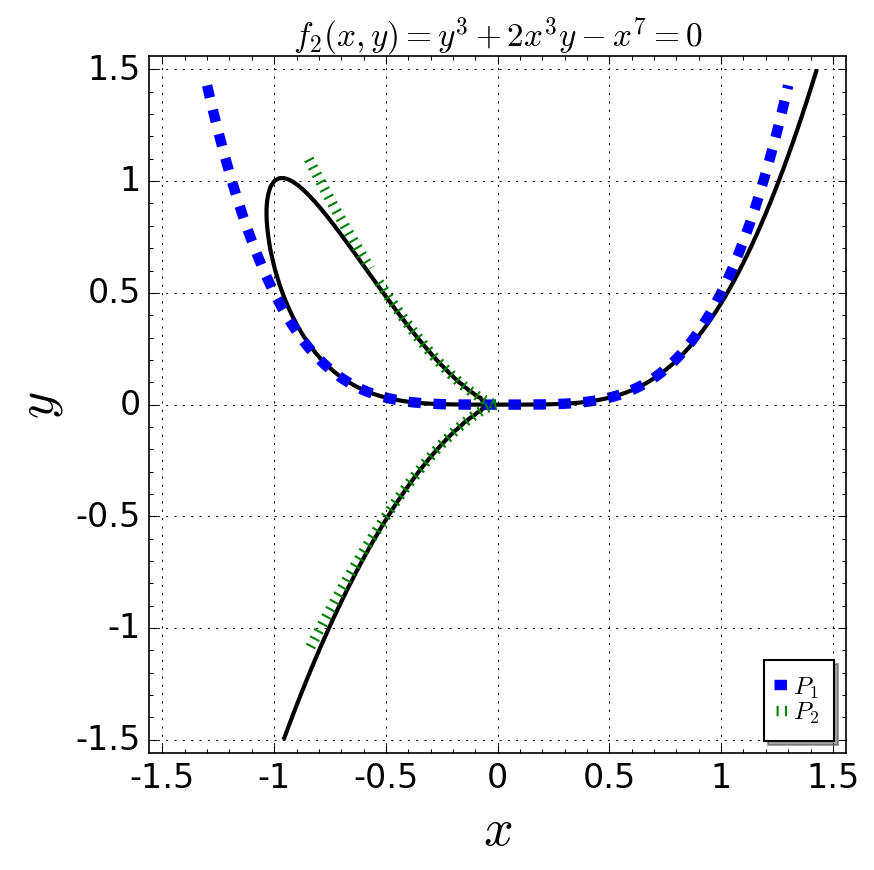
\includegraphics[width=0.49\textwidth]{images/f2-puiseux.png}
  \caption{A real plot of the curve $C_2: f_2(x,y) = y^3 + 2x^3y - x^7$. The
    blue and green dashed lines are plots of the places $P_1 = \left(t, t^4/2 +
      O(t^{9}) \right)$ and $P_2 = \left( -t^2/2, -t^3/2 + O(t^{8}) \right)$ for
    $t \in (-1.3, 1.3)$.}
  \label{fig:f2-puiseux}
  \end{figure}
  Again, the local parameter is always centered at $t=0$. Therefore, for small
  values of $|t|$ we see that $f_2\left(x(t), y(t)\right) = O(t^{19})$ is
  extraordinarily small in magnitude. As more terms are determined in the
  expansions of $y_1$ and $y_2$ we expect $N \to \infty$ in $f_2\left(x(t),
    y(t)\right) = O(t^N)$. We see that these series well-approximate the curve
  at $x=0$ in Figure \ref{fig:f2-puiseux}.
  
  We can verify these Puiseux series expansions above $x = 0$ and their
  properties using {\tt abelfunctions}.
  \begin{lstlisting}
  sage: P1, P2 = X2(0)  # the places above x=0 on the surface
  sage: P1
  (t, 1/2*t^4 + O(t^7))
  sage: P1.puiseux_series.extend(14)  # extend the curve to at least O(t^14)
  sage: P1
  (t, 1/2*t^4 - 1/16*t^9 + 3/128*t^14 + O(t^19))
  sage: P2
  (-1/2*t^2, -1/2*t^3 + O(t^5))
  sage: P2.puiseux_series.extend(13)  
  sage: P2  # may include higher order terms
  (-1/2*t^2, -1/2*t^3 - 1/64*t^8 + 3/4096*^13 - 1/16384*t^18 + O(t^20))
  \end{lstlisting}
\end{example}

\begin{example}
  Now consider the example curve,
  \[
    C_4 :  f_4(x,y) = x^2y^3 - x^4 + 1 = 0.
  \]
  \begin{figure}
  \centering
  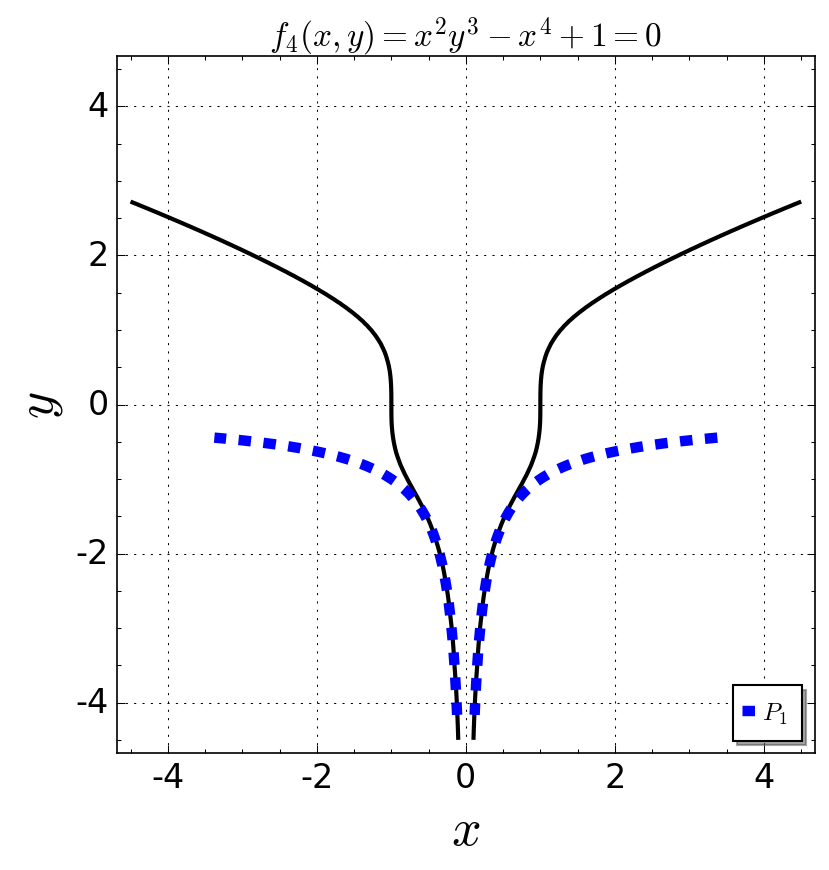
\includegraphics[width=0.49\textwidth]{images/f4-puiseux.png}
  \caption{A real plot of the curve $C_4: f_4(x,y) = x^2y^3 - x^4 + 1$. The
    dashed line is a plot of the place $P = \left(-t^3, -t^{-2} +
       O(t^{10})\right)$ for $t \in (-1.5, 1.5)$.}
  \label{fig:f4-puiseux}
  \end{figure}
  A plot of the curve in the real $x,y$-plane is shown in Figure
  \ref{fig:f4-puiseux}. There is a single place lying above $x=0$,
  \begin{equation}
    P(t) = \begin{cases}
      x(t) = -t^3, \\
      y(t) = -t^{-2} + \tfrac{1}{3}t^{10} + O(t^{15})
    \end{cases}
  \end{equation}
  Unlike the places shown in Example \ref{ex:f2-puiseux} the place $P$ has a
  component at infinity. The figure illustrates how $P$ acts as a local chart of
  the curve: the $O(t^{15})$ series expansion well-approximates the curve at
  $x=0$. In Abelfunctions, this place is treated like any other place.
  \begin{lstlisting}
  sage: P, = X4(0)
  sage: P  
  (-t^3, -t^-2 + O(t^0))
  sage: P.puiseux_series.extend(14)
  sage: P
  (-t^3, -t^-2 + 1/3*t^10 + O(t^15))
  \end{lstlisting}
\end{example}

Puiseux series expansions allow us to locally examine the behavior of an
algebraic curve or Riemann surface. In particular, they provide a local
coordinate chart centered at a point $(x,y) = (\alpha,\beta)$ on the curve in
the sense discussed in Section \ref{subsec:connection-to-riemann-surfaces}. In
the next section we describe a particular class of point/place on a Riemann
surface: the singular point.


%%%%%%%%%%%%%%%%%%%%%%%%%%%%%%%%%%%%%%%%%%%%%%%%%%%%%%%%%%%%%%%%%%%%%%%%%%%%%%%
\subsection{Singularities}\label{subsec:background-singularities}
%%%%%%%%%%%%%%%%%%%%%%%%%%%%%%%%%%%%%%%%%%%%%%%%%%%%%%%%%%%%%%%%%%%%%%%%%%%%%%%

Recall from Definition \ref{def: singular-point} that a point $a$ on a
projective curve $C$ is a singular point if
\[
  \left( \frac{\partial F}{\partial x_0}, \frac{\partial F}{\partial x_1},
    \frac{\partial F}{\partial x_2} \right) (a) = (0,0,0).
\]
For singular points of the form $a = (1 : \alpha, \beta)$, this is equivalent to
\[
  \frac{\partial f}{\partial x} (\alpha,\beta) = 0, \quad \frac{\partial
    f}{\partial y} (\alpha,\beta) = 0,
\]
where $f$ is the affine portion of the curve. The singular points of a curve
need to be determined not only for the numerical analytic continuation and
integration methods discussed below, so we can appropriately desingularize the
curve $C$ and obtain a Riemann surface $X$, but they are also an essential
ingredient to computing a basis of holomorphic 1-forms on $X$.

For singular points of the form $a = (1 : \alpha : \beta)$ the Puiseux series
expansion $P_j$ of $f = f(x,y)$ such that $P_j(0) = (\alpha, \beta)$ is a
coordinate chart centered at $(x,y) = (\alpha, \beta)$. $P_j$ tells us how to
approach and pass through $(x,y) = (\alpha, \beta)$ on the curve. Similarly,
singular points at infinity have coordinate charts defined by the Puiseux series
with $e_j < 0$. With these coordinate charts we can desingularize the curve and
thus create an appropriate atlas for the corresponding Riemann surface $X$.

For the purposes of later determining the genus of $X$ as well as the space of
holomorphic 1-forms $\Gamma(X,\Omega_X^1)$ on $X$ we need to compute the {\it
  delta invariant} and the {\it multiplicity} of a singularity. In the following
discussion we assume for simplicity that the singularity is finite. To analyze
infinite singular points we project the curve $C$ onto the line at infinity
$l_\infty$ using the method described in Section \ref{sec:
  projective-plane-curves}.

\begin{itemize}
\item {\bf branching number} --- The branching number $R$ of a singular point
  $(\alpha, \beta)$ is the sum of the branching numbers/ramification indices of
  the Puiseux series centered at $(x,y) = (\alpha,\beta)$. That is,
  \begin{equation} \label{eq:branching-number}
    R = \!\!\!\! \sum_{\substack{j \\ P_j(0)=(\alpha,\beta)}} |e_j|.
  \end{equation}
\item {\bf multiplicity} --- As given in Section \ref{sec:
    projective-plane-curves}, the multiplicity of a singular point is the degree
  of the lowest degree non-zero homogeneous term appearing in the polynomial
  expression for the curve centered at $(\alpha, \beta)$.
\item {\bf delta invariant} --- The delta invariant $\delta_P$ of a singularity
  $P$ is the number of double points concentrated at the singularity. This is
  equal to the number of quadratic factors $(\alpha_i x - \beta_i y)^2$
  appearing in the tangent cone at the singularity. Let $S$ be the set of all
  singular points, finite and infinity, of $C$. Then the genus is given by
  \begin{equation} \label{eq:genus-formula}
    g = \frac{(d-1)(d-2)}{2} - \sum_{P \in S} \delta_P.
  \end{equation}
\end{itemize}

\begin{example}
  We compute the singularities of the curve,
\[
  C_2 : f_2(x,y) = y^3 + 2x^3y - x^7 = 0.
\]
Note that to match the notation used in Sage the finite and infinite
singularities are presented in the format $(\alpha : \beta : 1)$ and $(\gamma :
1 : 0)$, respectively. The order of the projective components is different than
that presented in Section \ref{sec:projective-plane}.
\begin{lstlisting}
sage: S = singularities.singularities(f2)
sage: for s, (m, delta, r) in S:
....:     print 'Singularity:', s
....:     print '\tmultiplicity     =', m
....:     print '\tdelta invariant  =', delta
....:     print '\tbranching number =', r
....:
Singularity: (0, 0, 1)
	multiplicity     = 3
	delta invariant  = 4
	branching number = 2
Singularity: (0, 1, 0)
	multiplicity     = 4
	delta invariant  = 9
	branching number = 1
\end{lstlisting}
As seen in Equation \eqref{eq:f2-puiseux-series-expansions} the places $P_1$ and
$P_2$ above $x=0$, which have $y-$component $y(0) = 0$, have ramification
indices 1 and 2, respectively, which matches the expected multiplicity. HOLY
SHIT! THERE MAY BE AN ISSUE, HERE.

The genus is computed using the formula in Equation \eqref{eq:genus-formula}.
Later, performs additional checks on the genus using the geometric properties
discussed in \ref{subsec:background-monodromy}.
\begin{lstlisting}
sage: singularities.genus(f,x,y)
2  
\end{lstlisting}
\end{example}

\begin{example}
We compute the singularities of the curve,
\[
  C : f(x,y) = (y^2-x^2)(x-1)(2x-3) - 4(x^2+y^2-2x)^2.
\]
\begin{figure}
  \centering
  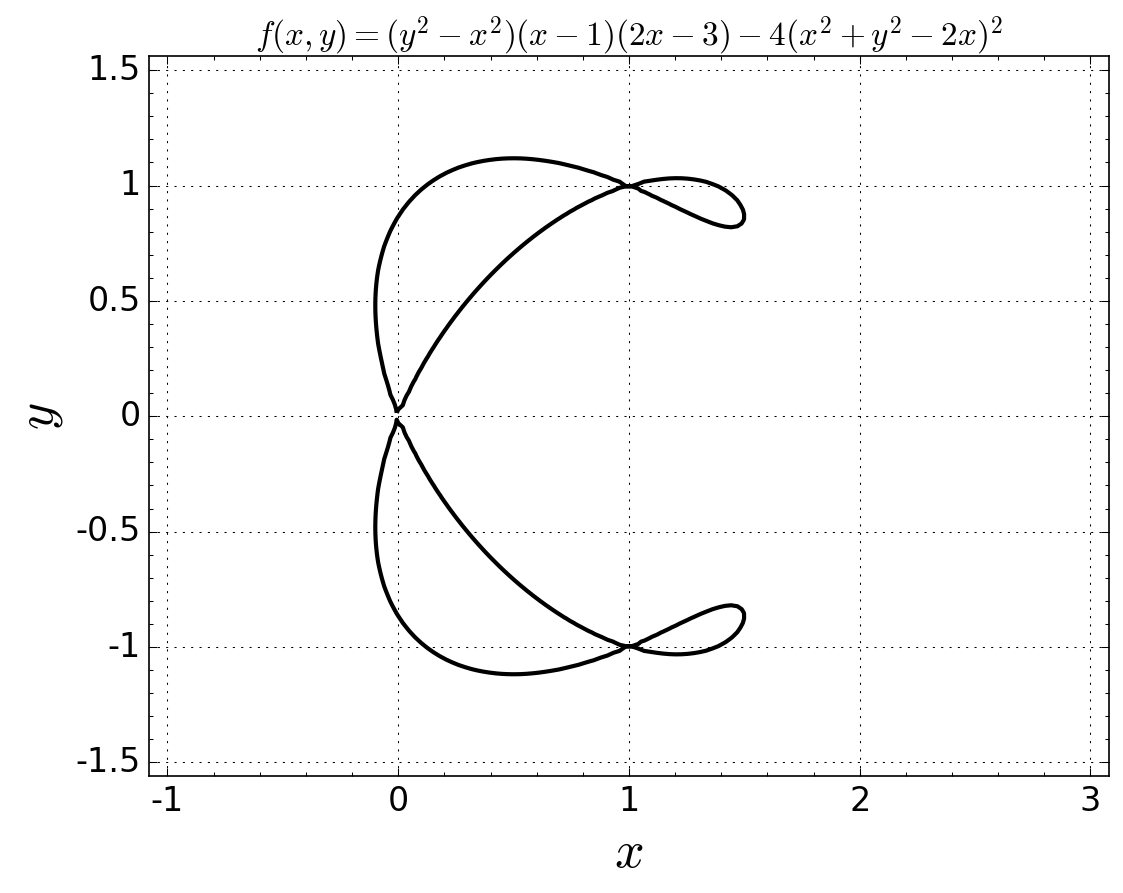
\includegraphics[width=0.49\textwidth]{images/f-singularities-example.png}
  \caption{A real plot of the curve $C: f(x,y) = (y^2-x^2)(x-1)(2x-3) -
    4(x^2+y^2-2x)^2$. Note the singularities at $(0,0), (1,1),$ and $(1,-1)$
    where the gradient vanishes.}
  \label{fig:f-singularities-example}
\end{figure}
A plot of the curve in the real $x,y$-plane is shown in Figure
\ref{fig:f-singularities-example}. The gradient of the curve in the affine plane
is given by,
\[
  \nabla f(x,y) = \left(
    -(12x-11)y^2 -24x^3 + 63x^2 - 38x, \quad
    -16y^3 - 2(6x^2 - 11x - 3)y
  \right).
\]
The gradient indeed vanishes at the points $(x,y) = (0,0), (1,1),$ and $(1,-1)$.
In fact, these are the only singular points of this curve.
\begin{lstlisting}
sage: f = (y^2-x^2)*(x-1)*(2*x-3) - 4*(x^2+y^2-2*x)^2
sage: S = singularities.singularities(f4)
sage: for s, (m, delta, r) in S:
....:     print 'Singularity:', s
....:     print '\tmultiplicity     =', m
....:     print '\tdelta invariant  =', delta
....:     print '\tbranching number =', r
....:
Singularity: (0, 0, 1)
	multiplicity     = 2
	delta invariant  = 1
	branching number = 2
Singularity: (1, -1, 1)
	multiplicity     = 2
	delta invariant  = 1
	branching number = 2
Singularity: (1, 1, 1)
	multiplicity     = 2
	delta invariant  = 1
	branching number = 2
\end{lstlisting}
This curve is a rational curve: the total degree of the curve is $d=4$ and the
three singularities have a delta invariant equal to one.
\end{example}


%%%%%%%%%%%%%%%%%%%%%%%%%%%%%%%%%%%%%%%%%%%%%%%%%%%%%%%%%%%%%%%%%%%%%%%%%%%%%%%
\subsection{Analytic Continuation} \label{subsec:background-analytic-continuation}
%%%%%%%%%%%%%%%%%%%%%%%%%%%%%%%%%%%%%%%%%%%%%%%%%%%%%%%%%%%%%%%%%%%%%%%%%%%%%%%

\begin{quote}
  The description of right lines and circles, upon which geometry is founded,
  belongs to mechanics. Geometry does not teach us to draw these lines, but
  requires them to be drawn. --- Isaac Newton
\end{quote}

The root of our geometric approach toward the period matrix of a Riemann surface
are paths on the Riemann surface. A {\it path on a Riemann surface, $X$,} is a
continuous map $\gamma : [0,1] \to X$. On the normalization of a curve $C:
f(x,y) = 0$ a path can be defined as $\gamma : [0,1] \to C \subset \CC^2$. In
particular, if $\gamma(t) = (x_\gamma(t), y_\gamma(t))$ then $f(x(t),y(t)) = 0$
for all $t \in [0,1]$ including points at infinity. Because the roots of a
polynomial are continuous as a function of the coefficients
\cite{HarrisMartin1987}, an $x$-path $x_\gamma : [0,1] \to \CC_x$ and an initial
$y$-root $y_0 \in \CC_y$ are sufficient for defining a path on $C$. Given these
information, the resulting $y$-path $y_\gamma : [0,1] \to \CC_y$ is completely
determined by the curve
\[
  f \big( x_\gamma(t), y_\gamma(t) \big) = 0, \quad y_\gamma(0) = y_0.
\]
The process of deriving this $y$-path from the data provided is called {\it
  analytic continuation}.

\begin{example}
A picture helps demonstrate this concept. Consider the curve,
\[
  C_2 : f_2(x,y) = y^3 + 2x^3y - x^7 = 0.
\]
Above $x=2$ are three unramified places, $y_0 = 4$, $y_1 = TODO$, and $y_2 =
TODO$. Consider the complex $x$-path $x_\gamma(t) = 2e^{i \pi t}$: the
counter-clockwise semi-circle of radius 2 centered at the origin beginning at
$x=2$. As $x$ continuously varies along this path for $t \in [0,1]$ the roots
$y_0 = y_{\gamma_0}(t)$, $y_1 = y_{\gamma_1}(t)$, and $y_2 = y_{\gamma_2}(t)$
vary continuously as well. Figure \ref{fig:ancont-c2-circle}

Consider, instead, the path $x_{\gamma} (t) = 2 - 4t$. Recall that $x=0$ has
three places lying above it each of them at $y=0$. To properly analytically
continue through this point along $x_{\gamma}$ we use the Puiseux series
expansions of $C$ at $x=0$ given in Equation
\eqref{eq:f2-puiseux-series-expansions},
\begin{align*}
    P_1(t) &= \begin{cases}
        x_1(t) = t, \\
        y_1(t) = \frac{t^{4}}{2} - \frac{t^{9}}{16} + \frac{3 t^{14}}{128} + O\left(t^{15}\right)
      \end{cases} \\
    P_2(t) &= \begin{cases}
      x_2(t) = - \frac{t^{2}}{2}, \\
      y_2(t) =  - \frac{t^{3}}{2} - \frac{t^{8}}{64} + \frac{3 t^{13}}{4096} + O\left(t^{14}\right)
    \end{cases}
\end{align*}
Figure \ref{fig: ancont-c2-line} shows how these three roots continuously ``pass
through'' the branch point.
  
\begin{figure}
  \begin{subfigure}[b]{0.48\textwidth}
    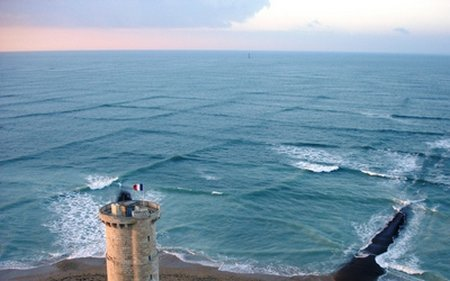
\includegraphics[draft,width=\textwidth]{images/livekp.jpg}
    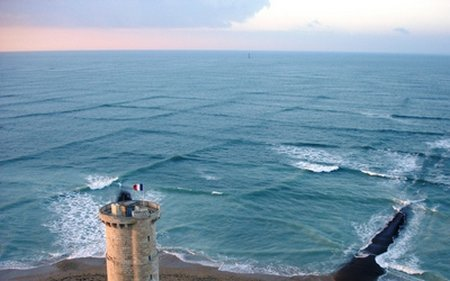
\includegraphics[draft,width=\textwidth]{images/livekp.jpg}
    \caption{$x_\gamma(t) = 2\exp(i \pi t)$}
    \label{fig:ancont-c2-circle}
  \end{subfigure}
  ~
  \begin{subfigure}[b]{0.48\textwidth}
    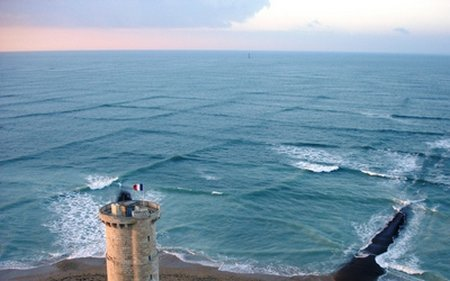
\includegraphics[draft,width=\textwidth]{images/livekp.jpg}
    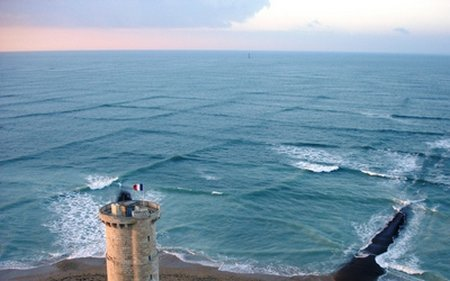
\includegraphics[draft,width=\textwidth]{images/livekp.jpg}
    \caption{$x_\gamma(t) = 2 - 4t$}
    \label{fig:ancont-c2-line}
  \end{subfigure}
  \caption{Analytic continuation of the roots $y_0 = 4, y_1 = TODO,$ and $y_1 =
    TODO$ of the curve $C_2$ along various paths in $\CC_x$.}
  \label{fig:ancont-c2}
\end{figure}
\end{example}

A {\it closed path $\gamma$ on a Riemann surface} is one such that $\gamma(0) =
\gamma(1)$. That is, a path is closed when $x_\gamma(0) = x_\gamma(1)$ and
$y_\gamma(0) = y_\gamma(1)$. When constructing a path using an $x$-path it may
be the case that the $x$-path $x_\gamma(t)$ is closed in $\CC_x$ but the derived
$y$-path $y_\gamma(t)$ may not satisfy $y_\gamma(0) = y_\gamma(1)$. This
situation is described in more detail in Section \ref{sec: monodromy} on
monodromy groups of algebraic curves. Finally, analytic continuation can be
extended to piecewise continuous path in $\CC_x$.


%%%%%%%%%%%%%%%%%%%%%%%%%%%%%%%%%%%%%%%%%%%%%%%%%%%%%%%%%%%%%%%%%%%%%%%%%%%%%%%
\subsection{Monodromy}\label{subsec:background-monodromy}
%%%%%%%%%%%%%%%%%%%%%%%%%%%%%%%%%%%%%%%%%%%%%%%%%%%%%%%%%%%%%%%%%%%%%%%%%%%%%%%

At a generic point $x = \alpha_0 \in \CC$ on a curve $C : f(x,y) = 0$ has $d$
distinct ordered $y$-roots $(y_0,\ldots,y_{d-1})$ at $\alpha_0$. This collection
of $y$-roots is sometimes called the {\it lift of} or the {\it fibre above}
$x=\alpha_0$. However, at a point $x=b$ where both $f(x,y) = 0$ and $\partial_y
f(x,y) = 0$ the number of distinct roots in the lift is strictly less than $d$.
Such a point $x = b$ is called a {\it discriminant point} of $f$. That is, a
discriminant point has at least one ramified place lying above it.

A {\it branch point} $x = b$ is a discriminant point having the property that if
one were to analytically continue a fibre around some closed path encircling $b$
then the elements of the fibre are permuted.

Specifically, let $x_{\gamma} : [0,1] \to \CC$ be a piecewise differentiable
oriented closed path in the complex $x$-plane encircling a branch point $x=b$
exactly once in the positive direction and let $(y_0, \ldots, y_{d-1})$ be a
fixed ordering of the fibre at $x_\gamma(0) = b$. Then, after analytically
continuing the fibre around $x_\gamma$ and returning to $x_\gamma(1) = b$, the
fibre is equal to
\begin{equation} \label{eq:permuted-fiber}
    (y_{\pi_b(0)}, \ldots, y_{\pi_b(d-1)}),
\end{equation}
where $\pi_b \in S_d$ is a permutation on $d$ elements. With this notation in
hand, a {\it branch point} is a discriminant point with $\pi_b \neq \text{id}$.

\begin{example}
  We see from the example in the previous section that the fibre $(y_0, y_1,
  y_2) = (2, TODO, TOO)$ above $x=2$ is permuted
\end{example}

To analyze the permutation behavior of multiple branch points
$\{b_1,\ldots,b_n\}$ we start by fixing some {\it base point} $x=\alpha_0$ in
the complex plane such that $\alpha_0$ is not a branch point and we fix an
ordering $(y_0,\ldots,y_{d-1})$ of the fibre above $\alpha_0$. Let $x_{\gamma_k}
: [0,1] \to \CC$ be a path encircling only the branch point $b_k$ in the
positive direction which does not cross the other paths. Such a path is called a
{\it monodromy path} of $b_k$. In the case when $x = \infty$ is a branch point a
monodromy path for $\infty$ is taken to be a circle going around all of the
finite branch points in the negative direction. See Figure \ref{fig: mon} for an
illustration of these paths.

\begin{figure}
  \centering
%  \includegraphics[width=0.6\textwidth]{images/mon.png}

  \begin{tikzpicture}
    \tikzstyle{discpt}=[circle,draw=white,fill=black,thin,minimum size=2pt,
                        radius=2pt]
    \tikzstyle{monpath}=[decoration={markings,
        mark=at position 0.5 with {\arrow[very thick]{latex}}},
      postaction={decorate}]

    % draw the discriminant points and interpolating dots
    \node[discpt] (b1) at (-1,-2)     [label=right:$b_1$] {};
    \node[discpt] (b2) at (0,-1)      [label=right:$b_2$] {};
    \node at (0,0) {$\bullet$};
    \node at (-0.1,0.4) {$\bullet$};
    \node at (-0.3,0.8) {$\bullet$};
    \node[discpt] (bn) at (-1,2)     [label=right:$b_n$] {};
    \node[discpt] (a) at (-6,0)      [label=left:$\alpha_0$] {};

    % the oriented paths
    \draw[monpath] (-6,0) ..
                   controls (-0.5,-3.5) and (0,-3) ..
                   (0,-2);
    \draw[monpath] (0,-2) ..
                   controls (0,-1) and (-2.5,-1.2) ..
                   (-6,0);
    \node at (-1.5,-2.8) {$x_{\gamma_1}$};

    \draw[monpath] (-6,0) ..
                   controls (-2.5,1.2) and (0,1) ..
                   (0,2);
    \draw[monpath] (0,2) ..
                   controls (0,3) and (-0.5,3.5) ..
                   (-6,0);
    \node at (-1.5,0.5) {$x_{\gamma_n}$};

    % path around infinity
    \draw[monpath] (-6,0) arc (180:0:4);
    \draw          (2,0) arc (0:-180:4);
    \node at (-4.5,2.8) {$x_{\gamma_\infty}$};

    %% \begin{scope}[very thick]
    %% \end{scope}
  \end{tikzpicture}
  \caption{The discriminant points $b_1,\ldots,b_n$ with their
    respective monodromy paths $x_{\gamma_1}, \ldots, x_{\gamma_n}$ and
    the path $x_{\gamma_\infty}$ around the point at infinity.}
  \label{fig: mon}
\end{figure}

Analytically continuing the ordered fibre $(y_0, \ldots, y_{d-1})$ around each
of the branch points results in $n+1$ permutations
\[
  \pi_{b_1}, \ldots, \pi_{b_n}, \pi_\infty \in S_d
\]
The group generated by these permutations is called the {\it fundamental group}
of $\CC \backslash \{b_1, \ldots, b_n\}$. It is denoted $\pi_1(\PP{1}\CC
\backslash \{b_1, \ldots, b_n\}, \alpha_0).$ Observe that, by the disjoint path
condition on the monodromy paths, moving the base point $\alpha_0$ corresponds
to conjugation of the generators of the fundamental group by some $\pi \in S_d$.
Hence, the monodromy group has explicit dependence on the base point.


We compute the monodromy group of the curve
\[
  C : f(x,y) = y^3 + 2x^3y - x^7 = 0,
\]
where the permutations $\pi_j \in \pi_1(\PP{1}\CC \backslash \{b_1, \ldots,
b_n\}, \alpha_0)$ are presented in disjoint cycle notation.
\begin{lstlisting}
from abelfunctions import *
from sympy.abc import x,y,t

f = y**3 + 2*x**3*y - x**7
X = RiemannSurface(f,x,y)

b = X.branch_points()
pi_1 = X.monodromy_group()

for bj,pi_1j in zip(b,pi_1):
    print 'branch point:', bj
    print 'permutation: ', pi_1j
    print
\end{lstlisting}
\begin{lstlisting}
branch point: (-0.31969776999-0.983928563571j)
permutation:  [(0, 2), (1,)]

branch point: (0.836979627962-0.608101294789j)
permutation:  [(0,), (1, 2)]

branch point: (-1.03456371594+0j)
permutation:  [(0,), (1, 2)]

branch point: 0j
permutation:  [(0, 2), (1,)]

branch point: (0.836979627962+0.608101294789j)
permutation:  [(0,), (1, 2)]

branch point: (-0.31969776999+0.983928563571j)
permutation:  [(0, 1), (2,)]

branch point: oo
permutation:  [(0, 2, 1)]
\end{lstlisting}
The method \verb=RiemannSurface.show_paths()= plots all the monodromy paths
$x_{\gamma_j}$ in the complex $x$-plane. The base point $x=\alpha_0$ is marked
in red.
\begin{lstlisting}[firstnumber=14]
X.show_paths()
\end{lstlisting}
\begin{lstlisting}
<matplotlib.figure.Figure object at 0x107d60810>
\end{lstlisting}
\begin{center}
%TODO \includegraphics[width=0.75\textwidth]{images/monexample.pdf}
\end{center}


%%%%%%%%%%%%%%%%%%%%%%%%%%%%%%%%%%%%%%%%%%%%%%%%%%%%%%%%%%%%%%%%%%%%%%%%%%%%%%%
\subsection{Homology}\label{subsec:background-homology}
%%%%%%%%%%%%%%%%%%%%%%%%%%%%%%%%%%%%%%%%%%%%%%%%%%%%%%%%%%%%%%%%%%%%%%%%%%%%%%%

A compact Riemann surface $X$ of genus $g$ is homeomorphic to a sphere with $g$
handles or, equivalently, a doughnut with $g$ holes. A cycle on $X$ is a closed,
oriented, piecewise smooth curve $\gamma : [0,1] \to X$ such that $\gamma(0) =
\gamma(1)$. The first homology group $H_1(X,\ZZ)$ of $X$ is the collection of
all cycles on $X$ modulo homologous transformations. In this document we do not
state precisely what it means for two cycles to be homologous since it involves
presenting the basic theory of simplicial complexes which is beyond the scope of
this document.

However, in brief, two cycles on $X$ are homologous if they can be deformed to
each other where the process of deformation not only allows continuous
transformations but the splitting of one cycle into two via ``pinching''. A
demonstration of this procedure is shown in Figure \ref{fig: pinching}. Two
cycles can be added together by ``reversing'' the pinching process and negation
of a path corresponds to reversing its orientation. The {\it first homology
  group} $H_1(X,\ZZ)$ is the set of all cycles on $X$ with the addition
operation described. The equivalence of cycles on a Riemann surface is the same
as that of closed paths on the complex plane (specifically, the Riemann sphere)
upon which one integrate a fixed meromorphic function $g$. Closed paths not
encircling a pole of $g$ are homologous to the zero path since they can be
contracted to a point. The set of all paths encircling a single, given pole are
all homologous to each other.

\begin{figure}
  \centering
  %
  % ONE BIG PATH
  \begin{tikzpicture}[scale=0.9]
    \colorlet{darkgreen}{green!50!gray}
    \colorlet{darkblue}{blue!50!gray}

    \begin{scope}[very thick]
    % Quadrant II of Torus
    % (other draw statements are flips / rotations)
    \draw (-6,0) ..
          controls (-6,1.5) and (-5,2.5) ..
          (-3.5,2.5) ..
          controls (-2,2.5) and (-1,1.5) ..
          (0,1.5);
    \draw[xscale=-1] (-6,0) ..
          controls (-6,1.5) and (-5,2.5) ..
          (-3.5,2.5) ..
          controls (-2,2.5) and (-1,1.5) ..
          (0,1.5);
    \draw[rotate=180] (-6,0) ..
          controls (-6,1.5) and (-5,2.5) ..
          (-3.5,2.5) ..
          controls (-2,2.5) and (-1,1.5) ..
          (0,1.5);
    \draw[yscale=-1] (-6,0) ..
          controls (-6,1.5) and (-5,2.5) ..
          (-3.5,2.5) ..
          controls (-2,2.5) and (-1,1.5) ..
          (0,1.5);

    % The Holes
    % (one hole at center shifted to outsides)
    \draw[xshift=-3.2cm] (-0.8,0) ..
          controls (-0.5,0.5) and (0.5,0.5) ..
          (0.8,0);
    \draw[yscale=-1,xshift=-3.2cm] (-1,-0.2) ..
          controls (-0.5,0.5) and (0.5,0.5) ..
          (1,-0.2);

    \draw[xshift=3.2cm] (-0.8,0) ..
          controls (-0.5,0.5) and (0.5,0.5) ..
          (0.8,0);
    \draw[yscale=-1,xshift=3.2cm] (-1,-0.2) ..
          controls (-0.5,0.5) and (0.5,0.5) ..
          (1,-0.2);

    % sum of paths example
    % gamma
    \draw[darkblue, decoration={markings,
              mark=at position 0.25 with {\arrow[very thick]{latex}}},
          postaction={decorate}]
    (0,0) ellipse (5cm and 0.9cm);
    \draw (0,-0.5) node {$\gamma$};
    \end{scope}
  \end{tikzpicture}

  \vspace{24pt}

  %
  % PINCHING THE PATHS
  %
  \begin{tikzpicture}[scale=0.9]
    \colorlet{darkgreen}{green!50!gray}
    \colorlet{darkblue}{blue!50!gray}

    \begin{scope}[very thick]
    % Quadrant II of Torus
    % (other draw statements are flips / rotations)
    \draw (-6,0) ..
          controls (-6,1.5) and (-5,2.5) ..
          (-3.5,2.5) ..
          controls (-2,2.5) and (-1,1.5) ..
          (0,1.5);
    \draw[xscale=-1] (-6,0) ..
          controls (-6,1.5) and (-5,2.5) ..
          (-3.5,2.5) ..
          controls (-2,2.5) and (-1,1.5) ..
          (0,1.5);
    \draw[rotate=180] (-6,0) ..
          controls (-6,1.5) and (-5,2.5) ..
          (-3.5,2.5) ..
          controls (-2,2.5) and (-1,1.5) ..
          (0,1.5);
    \draw[yscale=-1] (-6,0) ..
          controls (-6,1.5) and (-5,2.5) ..
          (-3.5,2.5) ..
          controls (-2,2.5) and (-1,1.5) ..
          (0,1.5);

    % The Holes
    % (one hole at center shifted to outsides)
    \draw[xshift=-3.2cm] (-0.8,0) ..
          controls (-0.5,0.5) and (0.5,0.5) ..
          (0.8,0);
    \draw[yscale=-1,xshift=-3.2cm] (-1,-0.2) ..
          controls (-0.5,0.5) and (0.5,0.5) ..
          (1,-0.2);

    \draw[xshift=3.2cm] (-0.8,0) ..
          controls (-0.5,0.5) and (0.5,0.5) ..
          (0.8,0);
    \draw[yscale=-1,xshift=3.2cm] (-1,-0.2) ..
          controls (-0.5,0.5) and (0.5,0.5) ..
          (1,-0.2);

    % sum of paths example
    % gamma_1
    \draw[darkblue, decoration={markings,
          mark=at position 0.4 with {\arrow[very thick]{latex}}},
          postaction={decorate}]
          (0,0) ..
          controls (3,-2) and (5,-2) ..
          (5,0);
    \draw[darkblue]
          (5,0) ..
          controls (5,2) and (3,2) ..
          (0,0);

    \draw[darkblue, decoration={markings,
          mark=at position 0.4 with {\arrow[very thick]{latex}}},
          postaction={decorate}]
          (0,0) ..
          controls (-3,2) and (-5,2) ..
          (-5,0);
    \draw[darkblue]
          (-5,0) ..
          controls (-5,-2) and (-3,-2) ..
          (0,0);
    \draw (0,-1.1) node {$\gamma$};
    \end{scope}
  \end{tikzpicture}

  \vspace{24pt}

  %
  % SEPARATING THE PATHS
  %
  \begin{tikzpicture}[scale=0.9]
    \colorlet{darkgreen}{green!50!gray}
    \colorlet{darkblue}{blue!50!gray}

    \begin{scope}[very thick]
    % Quadrant II of Torus
    % (other draw statements are flips / rotations)
    \draw (-6,0) ..
          controls (-6,1.5) and (-5,2.5) ..
          (-3.5,2.5) ..
          controls (-2,2.5) and (-1,1.5) ..
          (0,1.5);
    \draw[xscale=-1] (-6,0) ..
          controls (-6,1.5) and (-5,2.5) ..
          (-3.5,2.5) ..
          controls (-2,2.5) and (-1,1.5) ..
          (0,1.5);
    \draw[rotate=180] (-6,0) ..
          controls (-6,1.5) and (-5,2.5) ..
          (-3.5,2.5) ..
          controls (-2,2.5) and (-1,1.5) ..
          (0,1.5);
    \draw[yscale=-1] (-6,0) ..
          controls (-6,1.5) and (-5,2.5) ..
          (-3.5,2.5) ..
          controls (-2,2.5) and (-1,1.5) ..
          (0,1.5);

    % The Holes
    % (one hole at center shifted to outsides)
    \draw[xshift=-3.2cm] (-0.8,0) ..
          controls (-0.5,0.5) and (0.5,0.5) ..
          (0.8,0);
    \draw[yscale=-1,xshift=-3.2cm] (-1,-0.2) ..
          controls (-0.5,0.5) and (0.5,0.5) ..
          (1,-0.2);

    \draw[xshift=3.2cm] (-0.8,0) ..
          controls (-0.5,0.5) and (0.5,0.5) ..
          (0.8,0);
    \draw[yscale=-1,xshift=3.2cm] (-1,-0.2) ..
          controls (-0.5,0.5) and (0.5,0.5) ..
          (1,-0.2);

    % sum of paths example
    \draw[xshift=-3.2cm, darkblue, decoration={markings,
              mark=at position 0.25 with {\arrow[very thick]{latex}}},
          postaction={decorate}]
         (0,0) ellipse (2cm and 1.3cm);
    \draw[xshift=3.2cm, darkblue, decoration={markings,
              mark=at position 0.75 with {\arrow[very thick]{latex}}},
          postaction={decorate}]
         (0,0) ellipse (2cm and 1.3cm);

    \draw (0,-1.1) node {$\gamma = \gamma_1 + \gamma_2$};\
    \draw (-4,1.7)  node {$\gamma_1$};
    \draw (4,1.7)   node {$\gamma_2$};
    \end{scope}
  \end{tikzpicture}
  \caption{A genus $g=2$ Riemann surface $X$ with three homologous cycles. The
    process of ``pinching'' and separating a cycle $\gamma$ into two cycle is
    allowed. Cycles can be added together by reversing this pinching process.
    Negation of a cycle corresponds to reversing its orientation.}
  \label{fig: pinching}
\end{figure}

$H_1(X,\ZZ)$ has a basis of cycles $\{a_1,\ldots,a_g,b_1,\ldots,b_g\}$. That is,
every cycle on $X$ can be written as a finite, integer linear combination of the
$a$- and $b$-cycles. These cycles can be chosen such that they satisfy the
intersection properties
\begin{gather*}
  a_i \circ a_j = 0, \quad \forall i \neq j \\
  b_i \circ b_j = 0, \quad \forall i \neq j \\
  a_i \circ b_j = \delta_{ij}, \quad \forall i,j = 1, \ldots, g
\end{gather*}
where $\delta_{ij}$ is the Kronecker delta. That is, the only cycles that
intersect are $a_i$ and $b_i$. A basis of cycles fulfilling these intersection
requirements is called a {\it canonical basis of cycles}. Figure \ref{fig:
  cycle-basis} illustrates the canonical basis for a genus two Riemann surface.

\begin{figure}
  \centering
  %
  % DEMONSTRATION OF BASIS CYCLES
  %
  \begin{tikzpicture}
    \colorlet{darkgreen}{green!50!gray}
    \colorlet{darkblue}{blue!50!gray}

    \begin{scope}[very thick]
    % Quadrant II of Torus
    % (other draw statements are flips / rotations)
    \draw (-6,0) ..
          controls (-6,1.5) and (-5,2.5) ..
          (-3.5,2.5) ..
          controls (-2,2.5) and (-1,1.5) ..
          (0,1.5);
    \draw[xscale=-1] (-6,0) ..
          controls (-6,1.5) and (-5,2.5) ..
          (-3.5,2.5) ..
          controls (-2,2.5) and (-1,1.5) ..
          (0,1.5);
    \draw[rotate=180] (-6,0) ..
          controls (-6,1.5) and (-5,2.5) ..
          (-3.5,2.5) ..
          controls (-2,2.5) and (-1,1.5) ..
          (0,1.5);
    \draw[yscale=-1] (-6,0) ..
          controls (-6,1.5) and (-5,2.5) ..
          (-3.5,2.5) ..
          controls (-2,2.5) and (-1,1.5) ..
          (0,1.5);

    % The Holes
    % (one hole at center shifted to outsides)
    \draw[xshift=-3.2cm] (-0.8,0) ..
          controls (-0.5,0.5) and (0.5,0.5) ..
          (0.8,0);
    \draw[yscale=-1,xshift=-3.2cm] (-1,-0.2) ..
          controls (-0.5,0.5) and (0.5,0.5) ..
          (1,-0.2);

    \draw[xshift=3.2cm] (-0.8,0) ..
          controls (-0.5,0.5) and (0.5,0.5) ..
          (0.8,0);
    \draw[yscale=-1,xshift=3.2cm] (-1,-0.2) ..
          controls (-0.5,0.5) and (0.5,0.5) ..
          (1,-0.2);

    % a-cycles
    \draw[xshift=-3.2cm, darkblue, decoration={markings,
              mark=at position 0.25 with {\arrow[very thick]{latex}}},
          postaction={decorate}]
         (0,0) ellipse (2cm and 1.3cm);
    \draw[xshift=3.2cm, darkblue, decoration={markings,
              mark=at position 0.25 with {\arrow[very thick]{latex}}},
          postaction={decorate}]
         (0,0) ellipse (2cm and 1.3cm);

    % b-cycles
    \draw[xshift=-3.2cm, yshift=-2.47cm,
          darkgreen, decoration={markings,
              mark=at position 0.25 with {\arrow[very thick]{latex}}},
          postaction={decorate}]
         (0,0) arc (270:90:0.4cm and 1.07cm);
    \draw[xshift=-3.2cm, yshift=-0.33cm, dashed, darkgreen]
         (0,0) arc (90:-90:0.4cm and 1.07cm);
    \draw[xshift=3.2cm, yshift=-2.47cm,
          darkgreen, decoration={markings,
              mark=at position 0.25 with {\arrow[very thick]{latex}}},
          postaction={decorate}]
         (0,0) arc (270:90:0.4cm and 1.07cm);
    \draw[xshift=3.2cm, yshift=-0.33cm, dashed, darkgreen]
         (0,0) arc (90:-90:0.4cm and 1.07cm);

    % cycle labels
    \draw (-4,1.7)  node {$a_1$};
    \draw (4,1.7)   node {$a_2$};
    \draw (-3.2,-3) node {$b_1$};
    \draw (3.2,-3)  node {$b_2$};
    \end{scope}
  \end{tikzpicture}
  \caption{A genus $g=2$ Riemann surface $X$ with the basis cycles
    $\{a_1,a_2,b_1,b_2\}$ for the first homology group $H_1(X,\ZZ)$.}
  \label{fig: cycle-basis}
\end{figure}


We compute a homology basis for the Riemann surface $X$ obtained by
desingularizing and compactifying the curve
\[
  C : f(x,y) = y^3 + 2x^3y - x^7 = 0.
\]
The $a$- and $b$- cycles are presented as a list $[\ldots, s_i,(b_i,r_i),
s_{i+1}, \ldots]$ where $s_i$ is the current sheet number, $b_i$ is a branch
point of $C$, $r_i \in \ZZ$, and $s_{i+1}$ the the sheet reached after rotating
$r_i$ times around $b_i$ and returning to the base point $\alpha_0$.
\begin{lstlisting}
from abelfunctions import *
from sympy.abc import x,y,t

f = y**3 + 2*x**3*y - x**7
X = RiemannSurface(f,x,y)
a,b = X.homology()

# print the a-cycles
for i in range(g):
    print 'a_%d:'%(i+1)
    print a[i]
    print

# print the b-cycles
for i in range(g):
    print 'b_%d:'%(i+1)
    print b[i]
    print
\end{lstlisting}
\begin{lstlisting}
a_1:
[0, ((-0.31969776999025984-0.9839285635706635j), 1), 2,
 ((-1.0345637159435732+0j), -1), 1,
 ((-0.31969776999025984+0.9839285635706635j), -1), 0]

a_2:
[0, (0j, 1), 2, ((-0.31969776999025984-0.9839285635706635j), -1), 0]

b_1:
[0, ((-0.31969776999025984+0.9839285635706635j), 1), 1,
 ((0.8369796279620464-0.6081012947885316j), 1), 2,
 ((-0.31969776999025984-0.9839285635706635j), -1), 0]


b_2:
[0, ((-0.31969776999025984-0.9839285635706635j), 1), 2,
 ((-1.0345637159435732+0j), -1), 1,
 ((-0.31969776999025984+0.9839285635706635j), -1), 0, (oo, 1), 2,
 ((-0.31969776999025984-0.9839285635706635j), -1), 0,
 ((-0.31969776999025984+0.9839285635706635j), 1), 1,
 ((0.8369796279620464-0.6081012947885316j), 1), 2,
 ((-0.31969776999025984-0.9839285635706635j), -1), 0]
\end{lstlisting}

We can plot the projection of the cycle in the complex $x$- and $y$-planes. In
this example, we plot the cycle $a_1$ by computing 512 interpolating points on
the path. The $x$-projection $x_\gamma$ is in blue and the $y$-projection
$y_\gamma$ is in green.

\begin{lstlisting}
alpha = X.base_point()
betas = X.base_lift()
P0 = alpha, betas

gamma = RiemannSurfacePath((f,x,y), P0, cycle = a[0])
gamma.plot(512)
\end{lstlisting}
\begin{lstlisting}
<matplotlib.figure.Figure at 0x106e9cd90>
\end{lstlisting}
\begin{center}
%TODO \includegraphics[width=0.75\textwidth]{images/homexample.pdf}
\end{center}


%%%%%%%%%%%%%%%%%%%%%%%%%%%%%%%%%%%%%%%%%%%%%%%%%%%%%%%%%%%%%%%%%%%%%%%%%%%%%%%
\subsection{Holomorphic and Meromorphic
  Differentials}\label{subsec:background-holomorphic-and-meromorphic-differentials}
%%%%%%%%%%%%%%%%%%%%%%%%%%%%%%%%%%%%%%%%%%%%%%%%%%%%%%%%%%%%%%%%%%%%%%%%%%%%%%%

1-forms on a Riemann surface $X$ are objects that can be integrated along
piecewise smooth paths on $X$.
\begin{definition}
  {\bf (1-Form)} Let $X$ be a Riemann surface with atlas $\{ (U_\alpha,
  z_\alpha) \}$. A 1-form $\omega$ on $X$, also called a differential, is such
  that in each local coordinate $z_\alpha : U_\alpha \subset X \to \CC$,
  \[
    \omega \Big|_{U_\alpha} = f_\alpha(z_\alpha) dz_\alpha,
  \]
  and the appropriate compatibility conditions are satisfied under the action of
  transition functions on $U_\alpha \cup U_\beta$ where $(U_\beta, z_\beta)$ is
  another local coordinate. The space of all 1-forms on $X$ is denoted
  $\Omega_X^1$.
\end{definition}
The space of all {\it holomorphic 1-forms} is of particular interest.
\begin{definition}
  {\bf (Holomorphic 1-Forms)} The space of holomorphic 1-forms
  $\Gamma(X,\Omega_X^1)$ on $X$ is the space of 1-forms $\omega$ such that in
  each local coordinate $(U_\alpha, z_\alpha)$,
  \[
    \omega \Big|_{U_\alpha} = h_\alpha(z_\alpha) dz_\alpha
  \]
  where $h_\alpha : U_\alpha \to \CC$ is a holomorphic function.
\end{definition}
For a compact genus $g$ Riemann surface $X$, $\Gamma(X,\Omega_X^1)$ is a
finite-dimensional vector space of dimension $g$ over $\CC$. Thus, it has a
basis of $g$ holomorphic 1-forms $\{\omega_1, \ldots, \omega_g\}$.

For Riemann surfaces obtained by desingularizing and compactifying an algebraic
curve $C : f(x,y) = 0$ these basis holomorphic 1-forms can be written as
\begin{equation*}
  \omega_k(x,y) = \frac{p_k(x,y)}{\partial_y f(x,y)} dx,
\end{equation*}
where $p_k \in \CC[x,y]$ is of degree at most $d-3$ in $x$ and $y$. The
polynomials $p_k$ are called the {\it adjoint polynomials of $f$}. Note that
since $y$ has explicit dependence on $x$ due to the equation $f(x,y) = 0$, we
can use $x$ as the local coordinate of the differential.

We compute a basis of holomorphic 1-forms on the Riemann surface $X$ given by
the desingularization and compactification of the algebraic curve
\[
  C : f(x,y) = y^3 + 2x^3y - x^7 = 0.
\]
\begin{lstlisting}
from sympy.abc import x,y,t

f = y**3 + 2*x**3*y - x**7
X = RiemannSurface(f,x,y)
oneforms = X.holomorphic_differentials()

for omega in oneforms:
    print 'omega(x,y) =\n'
    sympy.pprint(omega, use_unicode=False)
    print
\end{lstlisting}
\begin{lstlisting}
omega(x,y) =

    x*y    
-----------
   3      2
2*x  + 3*y 

omega(x,y) =

      3    
     x     
-----------
   3      2
2*x  + 3*y
\end{lstlisting}
From this we can infer that the adjoint polynomials of the curve are $p_1(x,y) =
xy$ and $p_2(x,y) = x^3$.

%%%%%%%%%%%%%%%%%%%%%%%%%%%%%%%%%%%%%%%%%%%%%%%%%%%%%%%%%%%%%%%%%%%%%%%%%%%%%%%
\subsubsection{Divisors}\label{subsec:background-divisors}
%%%%%%%%%%%%%%%%%%%%%%%%%%%%%%%%%%%%%%%%%%%%%%%%%%%%%%%%%%%%%%%%%%%%%%%%%%%%%%%

The {\it valuation divisor} associated with a meromorphic one-form on $X$ is a
direct ingredient in the determination of finite-genus solutions to the
KP-equation. Before we define the valuation divisor we take a brief detour into
the realm of general divisors on a Riemann surface.

\begin{definition}
  A {\bf divisor} $\DivD$ on the Riemann surface $X$ is a finite formal linear
  combination of places $P_i$ with multiplicities $n_i$:
  \begin{equation}
    \DivD = \sum_i n_i P_i.
  \end{equation}
  The sum,
  \begin{equation}
    \deg \DivD = \sum_i n_i
  \end{equation}
  is called the {\bf degree of $\DivD$}.
\end{definition}
The set of all divisors on a Riemann surface forms an Abelian group
$\text{Div}(X)$ under addition. A divisor with all $n_i \geq 0$ is called {\it
  positive} or {\it effective}.



%%%%%%%%%%%%%%%%%%%%%%%%%%%%%%%%%%%%%%%%%%%%%%%%%%%%%%%%%%%%%%%%%%%%%%%%%%%%%%%
\subsection{Jacobian and Period
  Matrices}\label{subsec:background-jacobian-and-period-matrices}
%%%%%%%%%%%%%%%%%%%%%%%%%%%%%%%%%%%%%%%%%%%%%%%%%%%%%%%%%%%%%%%%%%%%%%%%%%%%%%%

Period matrices are matrices obtained by integrating the holomorphic
differentials $\omega_1, \ldots, \omega_g$ along the $a$-cycles $a_1,\ldots,a_g$
and $b$-cycles $b_1,\ldots,b_g$. Define the $g \times g$ matrices
\begin{align*}
  A = \left( A_{ij} \right)_{i,j=1}^g,
  \quad A_{ij} = \oint_{a_j} \omega_i, \\
  B = \left( B_{ij} \right)_{i,j=1}^g,
  \quad B_{ij} = \oint_{b_j} \omega_i.
\end{align*}
A {\it period matrix} of $X$ is the $g \times 2g$ matrix
\[
  \tau = \left[ A \; B \right].
\]
We often normalize the differentials $\omega_i$ such that $A_{ij} = \delta_{ij}$
which results in the period matrix
\begin{equation} \label{eqn: period-matrix}
  \tau = \left[ I_{g \times g} \; \Omega \right].
\end{equation}
This is equivalent to setting $\Omega = A^{-1}B$. The matrix $\Omega \in \CC^{g
  \times g}$ is a {\it Riemann matrix}: an invertible, symmetric complex matrix
with positive definite imaginary part. The columns of $\tau$ define a lattice
\[
  \Lambda = \{I m + \Omega n \; | \; m,n \in \ZZ^g\} \subset \CC^g.
\]
This lattice plays an important role in the theory of algebraic curves since the
quotient space
\begin{equation} \label{eqn: jacobian}
  J(C) = \CC^g / \Lambda \cong \mathbb{T}^{2g}
\end{equation}
is the {\it Jacobian} or {\it Jacobian variety} of the curve $C$. Jacobian
varieties play a central role in the theory of algebraic curves. For example,
the Torelli theorem \cite{Mumford99} states that a non-singular projective curve
is completely determined by its Jacobian. The Schottky problem establishes a
link between the Jacobian and the Kadomtsev--Petviashvili equation by providing
conditions on when a given Riemann matrix is a period matrix of some algebraic
curve.

%TODO Schottky problem

The \verb=RiemannSurface.period_matrix()= method returns the matrices $A$ and
$B$ defined above. The Riemann matrix $\Omega$ is obtained by computing $\Omega
= A^{-1}B$

\begin{lstlisting}
from abelfunctions import *
from sympy.abc import x,y,t
from scipy import dot
from scipy.linalg import inv

f = -x**7 + 2*x**3*y + y**3
X = RiemannSurface(f, x, y)
A,B = X.period_matrix()
Omega = dot(inv(A), B)

print 'A =\n', A
print 'B =\n', B
print 'Omega =\n', Omega
\end{lstlisting}
\begin{lstlisting}
A =
[[ -1.38142275e-12-1.20192474j   1.84957199e+00+0.60096237j]
 [  9.22903420e-12+1.97146395j   7.16176201e-01-0.98573197j]]
B =
[[-0.70647363+2.17430227j -1.84957199+2.54571744j]
 [-1.87497364-1.36224808j -0.71617620+0.23269975j]]
Omega =
[[-1.30901699+0.95105652j -0.80901699+0.58778525j]
 [-0.80901699+0.58778525j -1.00000000+1.1755705j ]]
\end{lstlisting}
We numerically verify that $\Omega$ is a Riemann matrix by computing $\|\Omega -
\Omega^T\|$ as well as the eigenvalues of $\im \Omega$.
\begin{lstlisting}[firstnumber=14]
print norm(Omega.T - Omega)
print
print eigvals(Omega.imag)
\end{lstlisting}
\begin{lstlisting}
9.303308740879998e-11

[ 0.46490467  1.66172235]
\end{lstlisting}


%%%%%%%%%%%%%%%%%%%%%%%%%%%%%%%%%%%%%%%%%%%%%%%%%%%%%%%%%%%%%%%%%%%%%%%%%%%%%%%
\subsection{The Abel Map}\label{subsec:background-the-abel-map}
%%%%%%%%%%%%%%%%%%%%%%%%%%%%%%%%%%%%%%%%%%%%%%%%%%%%%%%%%%%%%%%%%%%%%%%%%%%%%%%

\begin{definition}\label{def:abelmap}
  Let $P \in X$ be a fixed place. The Abel Map $\boldsymbol{A} : X \to
  J(X)$ is defined by
  \begin{equation} \label{eqn:abel1}
    \boldsymbol{A}(P,Q) = \big( A_1(P,Q), \ldots, A_g(P,Q) \big),
  \end{equation}
  where
  \begin{equation} \label{eqn:abel2}
    A_j(P,Q) = \int_P^Q \omega_j,
  \end{equation}
  and the path chosen from $P$ to $Q$ is the same for each $A_j$. The
  Abel map is written in vector form as
  \begin{equation} \label{eqn:abel-vector}
    \boldsymbol{A}(P,Q) = \int_P^Q \boldsymbol{\omega}.
  \end{equation}
\end{definition}
The definition of the Abel map can be extended to divisors: let $\DivD =
\sum_i n_i P_i$. We define
\begin{equation} \label{eqn:abel-divisors}
  \boldsymbol{A}(P,\DivD) = \sum_i n_i \boldsymbol{A}(P,P_i).
\end{equation}
The Abel Map is independent of the path $\gamma$ from $P$ to $Q$ chosen
on $X$ for if $\gamma$ and $\eta$ are two such paths then their
difference is a linear combination of homology basis cycles. The
integral of $\boldsymbol{\omega}$ along this closed path is a lattice
element and therefore is congruent to zero in $J(X)$.

An algorithm for computing the Abel map is described in
\cite{DeconinckPatterson11}. The implementation in {\sc abelfunctions}
is based on this algorithm.

\begin{example}
{\sc abelfunctions} selects a regular ``base place'' $P_0$ from which to
construct all paths on $X$. When given a single argument {\tt AbelMap()}
returns $\Abel(P_0,P)$.
\begin{lstlisting}
sage: J = Jacobian(X)       # reduces vectors modulo lattice ZZ^g + Omega ZZ^g
sage: z1 = AbelMap(P); z1   # Abel map from P0 to P
[-0.5261+0.0864j  0.0669+0.6392j -0.7495+1.1037j -1.5030+1.0356j]
sage: z2 = AbelMap(Q); z2   # Abel map from P0 to Q
[-0.3875+0.1157j -0.0290+0.4437j -0.4532+0.7774j -0.9721+0.6732j]
sage: z3 = AbelMap(P,Q); z3 # Abel map from P to Q
[ 0.1468-0.0985j  0.8467+0.6989j  0.0996+1.0083j -1.1003+0.8159j]
sage: numpy.linalg.norm( J((z2-z1) - z3) ) # numerically verify that A(P,Q) = A(P0,Q) - A(P0,P)
3.80631643473e-16
\end{lstlisting}
The Abel map accepts divisors as well.
\begin{lstlisting}
sage: w = AbelMap(D); w
[ 0.0670-0.1361j  0.9421+0.7429j -0.4887+0.7663j -1.5057+0.6992j]
sage: z = J(3*z1 + z2) # verify that w = 3*z1 + z2 mod period lattice
sage: numpy.linalg.norm(w-z)
1.57107346e-15
\end{lstlisting}
\end{example}


%%%%%%%%%%%%%%%%%%%%%%%%%%%%%%%%%%%%%%%%%%%%%%%%%%%%%%%%%%%%%%%%%%%%%%%%%%%%%%%
\subsection{The Riemann Constant
  Vector}\label{subsec:background-the-riemann-constant-vector}
%%%%%%%%%%%%%%%%%%%%%%%%%%%%%%%%%%%%%%%%%%%%%%%%%%%%%%%%%%%%%%%%%%%%%%%%%%%%%%%

\begin{definition} \label{def:rcv}
Let $X$ be a genus $g$ Riemann surface with associated Riemann matrix
$\Omega$. The Riemann constant vector $\RCV : X \to J(X)$ is defined as
\begin{equation} \label{eqn:rcv1}
  \RCV(P) = \big( K_1(P), \ldots, K_g(P) \big),
\end{equation}
where
\begin{equation} \label{eqn:rcv2}
  K_j(P) = \frac{1 + \Omega_{jj}}{2} - \sum_{k \neq j}^g
           \oint_{a_k} \omega_k(Q) A_j(P,Q).
\end{equation}
\end{definition}
Once we know the value of $\RCV(P_0)$ the value of $\RCV(P)$ is
determined using only a shift by the Abel map:
\begin{theorem} \label{thm:RCVshift}
  Let $P_0,P$ be places on a genus $g$ Riemann surface $X$. Then
  \begin{equation} \label{eqn:RCVshift}
    \RCV(P) = \RCV(P_0) + (g-1)\Abel(P_0,P).
  \end{equation}
\end{theorem}
\begin{proof}
Let $Q$ be an arbitrary place on $X$. By the definition of the Abel map,
$\Abel(P,Q) = \Abel(P,P_0) + \Abel(P_0,Q)$. Using this identity in the
definition of the RCV we obtain
\begin{align} \label{eqn:RCVshift1}
  K_j(P)
  &=
  \frac{1 + \Omega_{jj}}{2}
  -
  \sum_{k \neq j}^g
  \oint_{a_k} \omega_k(Q) A_j(P,Q) \dQ  \notag \\
  &=
  \frac{1 + \Omega_{jj}}{2}
  -
  \sum_{k \neq j}^g
  \oint_{a_k} \omega_k(Q) \Big( A_j(P,P_0) + A_j(P_0,Q) \Big) \dQ  \notag \\
  &=
  \frac{1 + \Omega_{jj}}{2}
  -
  \sum_{k \neq j}^g
  \oint_{a_k} \omega_k(Q) A_j(P,P_0) \dQ
  -
  \sum_{k \neq j}^g
  \oint_{a_k} \omega_k(Q) A_j(P_0,Q) \dQ.
\end{align}
The $j$th-component of the Abel map appearing in the first sum has no
dependence on the variable of integration $Q$ nor on the summation index
$k$. Therefore,
\begin{align} \label{eqn:RCVshift2}
  K_j(P)
  &=
  \frac{1 + \Omega_{jj}}{2}
  -
  A_j(P,P_0)
  \sum_{k \neq j}^g
  \oint_{a_k} \omega_k(Q) \dQ
  -
  \sum_{k \neq j}^g
  \oint_{a_k} \omega_k(Q) A_j(P_0,Q) \dQ \notag \\
  &=
  \frac{1 + \Omega_{jj}}{2}
  -
  A_j(P,P_0) (g-1)
  -
  \sum_{k \neq j}^g
  \oint_{a_k} \omega_k(Q) A_j(P_0,Q) \dQ \notag \\
  &=
  K_j(P_0) + (g-1)A_j(P_0,P).
\end{align}
\end{proof}
The primary computational benefit to using the result of Theorem
\ref{thm:RCVshift} is that most of the work in evaluating $\RCV$ comes
from evaluating it at a fixed place $P_0$. Once this is done, we only
need the Abel map to determine $\RCV$ for all other places $P \in X$. In
{\sc abelfunctions} a fixed place of the Riemann surface is
automatically chosen.

The inspiration behind the algorithm for computing the RCV described in
the following section comes from the following two theorems. Theorem
\ref{thm:rcvequiv} characterizes a certain class of divisors in terms of
the RCV, a proof of which is found in \cite{FarkasKra92}.
\begin{theorem} \label{thm:rcvequiv}
  Let $\DivC$ be a divisor on a genus $g$ Riemann surface $X$ of degree
  $2g - 2$. Then $\DivC$ is a canonical divisor if and only if
  \begin{equation} \label{eqn:rcvequiv}
    2\RCV(P) \equiv -\Abel(P,\DivC).
  \end{equation}
\end{theorem}
\noindent Theorem \ref{thm:thetadivisor} establishes a connection
between the Riemann theta function and the RCV, a proof of which is also
found in \cite{FarkasKra92}.
\begin{definition} \label{def:riemanntheta}
  The Riemann theta function $\theta: J(X) \times \hg \to \CC$ is
  defined by
  \begin{equation} \label{eqn:riemanntheta}
    \theta(z,\Omega)
    =
    \sum_{n \in \ZZ^g}
    e^{2 \pi i \left( \tfrac{1}{2} n \cdot \Omega n + n \cdot z \right)}.
  \end{equation}
  This series converges absolutely and uniformly on compact sets in
  $J(X) \times \hg$ where $\hg$ is the space of all Riemann matrices.
\end{definition}

\begin{theorem} \label{thm:thetadivisor}
  Let $\Omega$ be the Riemann matrix associated with the Riemann surface
  $X$ and $P_0 \in X$ an arbitrary place. Then a vector $\boldsymbol{W}
  \in J(X)$ satisfies
  \begin{equation} \label{eqn:thetadivisor1}
    \theta(\boldsymbol{W}, \Omega) = 0,
  \end{equation}
  if and only if there exists a divisor $\DivD = P_1 + \cdots P_{g-1}$
  such that
  \begin{equation} \label{eqn:thetadivisor2}
    \boldsymbol{W} = \boldsymbol{A}(P_0, \DivD) + \boldsymbol{K}(P_0).
  \end{equation}
\end{theorem}
Note that $\DivD$ may contain a place of multiplicity greater than
one. The primary requirement of $\DivD$ is that it is of degree $g-1$
and is effective. The set $\Theta := \{ \boldsymbol{W} \in J(X) :
\theta(\boldsymbol{W},\Omega) = 0\}$ is known as the {\it theta divisor}
of the Riemann surface $X$. It is a $(g-1)$ complex--dimensional
subvariety of $J(X)$. Theorem \ref{thm:thetadivisor} states that $\Theta
= \Abel\left(P_0,SX^{g-1}\right) + \boldsymbol{K}(P_0)$ where $SX^{g-1}$
is the $(g-1)$--fold symmetric product of the Riemann surface.


%%%%%%%%%%%%%%%%%%%%%%%%%%%%%%%%%%%%%%%%%%%%%%%%%%%%%%%%%%%%%%%%%%%%%%%%%%%%%%%
\section{The Riemann Theta
  Function}\label{sec:background-riemann-theta-function}
%%%%%%%%%%%%%%%%%%%%%%%%%%%%%%%%%%%%%%%%%%%%%%%%%%%%%%%%%%%%%%%%%%%%%%%%%%%%%%%